
\appendix

\section{Generalized Causal Attention}\label{appendix:secA}
We design the Generalized Causal Attention for CausalFusion models. The core idea is to maintain causal dependencies across all AR steps while ensuring that each AR step relies only on \textit{clean} image tokens from preceding AR steps. This design allows CausalFusion to generate images using a \textit{next-token(s) diffusion} paradigm.
We show an example of the generalized causal attention mask in Figure~\ref{fig:generalized_causal_mask}, and the PyTorch-style pseudo code for obtaining generalized causal mask in Algorithm~\ref{algo:gcm}.

\begin{figure}[h]\centering
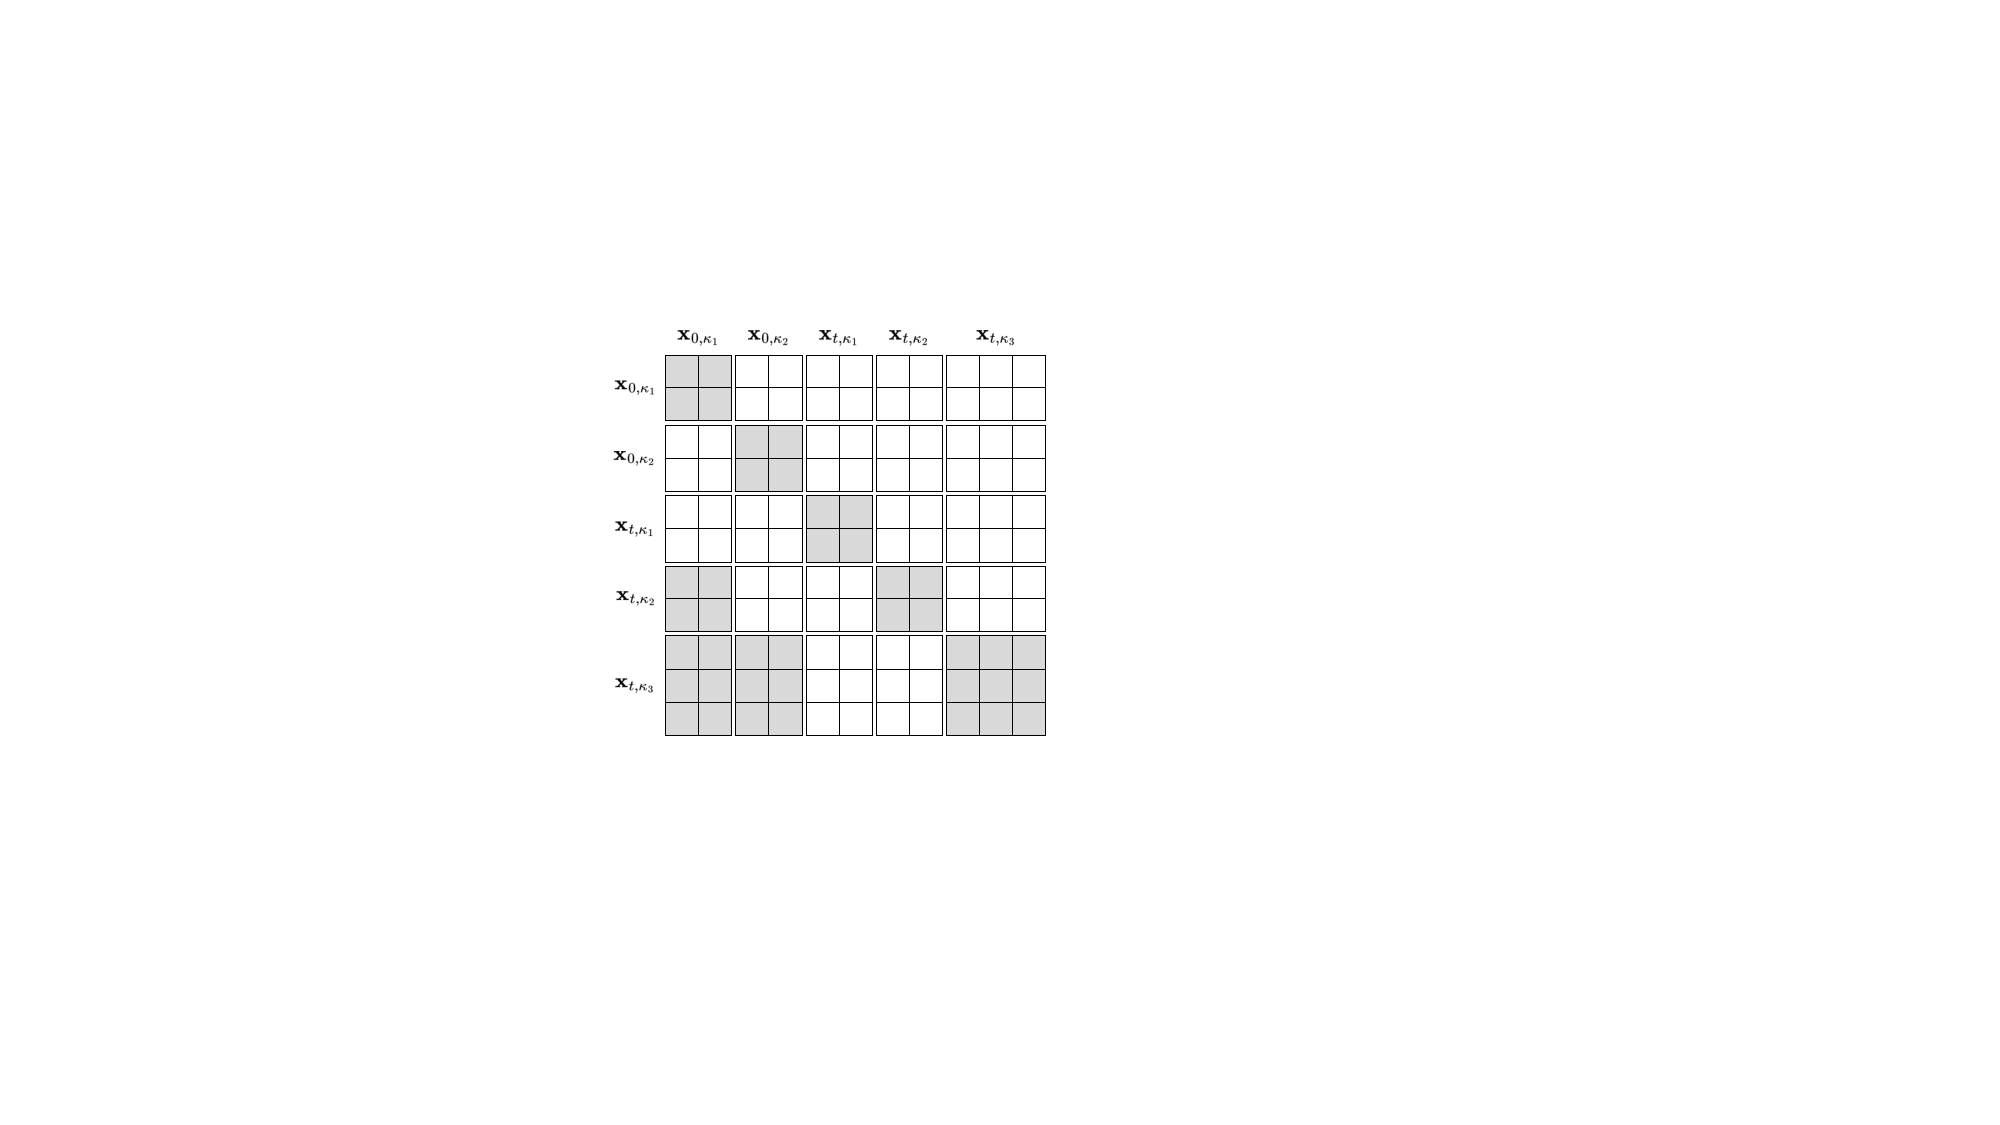
\includegraphics[width=0.7\linewidth]{figs/gca.pdf}
\vspace{-5pt}
\caption{\textbf{Generalized causal mask.} In this case, the input sequence is organized to have 3 AR-steps $\kappa_1$, $\kappa_2$, and $\kappa_3$, containing 2, 2, and 3 tokens, respectively. $\mathbf{x}_{0, \kappa_1}$ and $\mathbf{x}_{0, \kappa_2}$ are the clean tokens at the first two AR steps, while $\mathbf{x}_{t, \kappa_1}$, $\mathbf{x}_{t, \kappa_2}$, and $\mathbf{x}_{t, \kappa_3}$ are noised tokens. White and gray blocks denote the masked and unmasked attention, respectively. Note that, each $\mathbf{x}_{t, \kappa_s}$ only attends to itself and the clean tokens from previous AR steps $\mathbf{x}_{0, \kappa_{1:s-1}}$.}
\label{fig:generalized_causal_mask}
\end{figure}
\vspace{-10pt}


\section{More Analyses}\label{appendix:secB}
\paragraph{Diffusion time steps sampling.}
Following DiT~\cite{dit}, we randomly sample the diffusion time step $t$ during training. By default, the same $t$ is used across all AR steps when training CausalFusion models. Here, we explore the impact of using different $t$ values for different AR steps during training. The training and evaluation settings remain consistent with Section~\ref{sec:init_exps}. As shown in Table~\ref{tab:timestep}, using either shared or random $t$ values results in similar performance, indicating that CausalFusion is robust to this variation.
Additionally, we evaluate a setting where multiple diffusion time steps are sampled for each AR step. Specifically, we experiment with sampling 4 and 8 different time steps, reducing the batch size by factors of 4$\times$ and 8$\times$, respectively, to ensure the total number of tokens used for loss calculation remains constant. As shown in the table, using multiple diffusion time steps per AR step achieves comparable performance to the default setting, further demonstrating the robustness of CausalFusion to this factor.
Notably, in this approach, the clean image tokens $\mathbf{x}_{0, \kappa{s}}$ at each AR step need to be computed only once and can be shared across multiple $\mathbf{x}_{t, \kappa_s}$ with different $t$ values. Consequently, the additional computational cost introduced by clean image tokens during training is minimized, amounting to only $\sim$10\%.
\vspace{-5pt}

\begin{algorithm}[t]
\caption{
Generalized causal mask}
\label{algo:gcm}
\definecolor{codeblue}{rgb}{0.25,0.5,0.5}
\definecolor{codekw}{rgb}{0.85, 0.18, 0.50}
\begin{lstlisting}[language=python]
def get_attn_mask(ctx_len, x_len, step):
    # tx_len: the length of clean tokens
    # x_len: the length of noisy tokens
    # step: number of AR steps

    # sample random tokens per AR step
    sumk = random.sample(range(1, x_len), step - 1)
    sumk = [0] + sorted(sumk) + [x_len]

    # build `causal` masks
    seq_len = ctx_len + x_len
    attn_mask = torch.ones(size=(seq_len, seq_len))
    m1 = torch.ones(size=(ctx_len, ctx_len))
    m2 = torch.ones(size=(x_len, ctx_len))
    m3 = torch.ones(size=(x_len, x_len))
    for i in range(len(sumk) - 2):
        m1[sumk[i]:sumk[i+1], 0:sumk[i+1]] = 0
        m2[sumk[i+1]:sumk[i+2], 0:sumk[i+1]] = 0
    for i in range(len(sumk) - 1):
        m3[sumk[i]:sumk[i+1], sumk[i]:sumk[i+1]] = 0

    attn_mask[:ctx_len, :ctx_len] = m1
    attn_mask[ctx_len:, :ctx_len] = m2
    attn_mask[ctx_len:, ctx_len:] = m3
    return attn_mask # 1 for mask, 0 for unmask
\end{lstlisting}
\end{algorithm}


\begin{table}[h]
\footnotesize
\centering
\begin{tabular}{c|c}
& FID10k\\ 
\shline
\underline{shared $t$ for different AR steps} & 12.13 \\
random $t$ for different AR steps & 12.27 \\
4$\times$ $t$ for each AR step & 12.19 \\
8$\times$ $t$ for each AR step & 12.23 \\
\end{tabular}
\vspace{-5pt}
\caption{\textbf{Diffusion time steps sampling} strategy does not affect the performance. The default setting is \underline{underlined}.}
\label{tab:timestep}
\end{table}
\vspace{-10pt}

\begin{table}[h]
\footnotesize
\centering
\begin{tabular}{c|cc}
\#class tokens & params (M) & FID10k\\ 
\shline
\underline{4} & 308 (+3.9) &  12.13 \\
16 & 320 (+15.6) &  12.04 \\
{64} & 368 (+62.5) &  11.84 \\
1 (repeat 64$\times$) & 305 (+1.0) & 12.29  \\
4 (repeat 16$\times$) & 308 (+ 3.9) & \textbf{11.75}  
\end{tabular}
\vspace{-5pt}
\caption{\textbf{\#Class tokens} offers a trade-off between performance and number of parameters. The default setting is \underline{underlined}.}
\label{tab:cls-token}
\end{table}
\vspace{-15pt}

\paragraph{Class condition tokens.} As discussed in Sections~\ref{sec:init_exps} and \ref{sec:sota_exp}, we use 4 class condition tokens for ablation studies and 64 tokens for system-level comparisons. Here, we examine the impact of the number of class tokens in the CausalFusion framework. As shown in Table~\ref{tab:cls-token}, increasing the number of class tokens to 64 slightly improves performance (12.13 vs. 11.84 FID). However, this also adds 62.5M parameters, a significant increase (20\%) for a CausalFusion-L model with 304M parameters. To address this, we adopt a token-repeating strategy from~\cite{mar}, which achieves comparable performance (11.75 vs. 11.84 FID) without increasing the parameter count. This finding suggests that the computation allocated to class conditioning is more critical than the number of parameters dedicated to it.


\section{Implementation Details}\label{appendix:secC}
\label{appendix:impl}

\paragraph{Class-conditional image generation.} In Table~\ref{tab:impl_abla}, we provide the detailed settings of CausalFusion models for class-conditional image generation in Section~\ref{sec:init_exps} and \ref{sec:difficulty}.
\vspace{-5pt}

\begin{table}[h]
    \footnotesize
    \begin{tabular}{c|c}
        config & value \\
        \shline
        image resolution & 256$\times$256 \\
        hidden dimension & 1024 \\
        \#heads & 16 \\
        \#layers & 24 \\
        \#cls tokens & 4 \\
        patch size & 2 \\
        positional embedding & sinusoidal \\
        VAE & SD~\cite{SD-vae} \\
        VAE donwsample& 8$\times$ \\
        latent channel & 4 \\
        \hline
        optimizer & AdamW~\cite{loshchilov2017decoupled} \\
        base learning rate & 1e-4 \\
        weight decay & 0.0 \\
        optimizer momentum & $\beta_1, \beta_2{=}0.9, 0.95$ \\
        batch size & 2048 \\
        learning rate schedule & constant \\
        warmup epochs & 40 \\
        training epochs & 240 \\
        augmentation & horizontal flip, center crop \\
        \hline
        diffusion sampler & DDPM~\cite{ddpm} \\
        diffusion steps & 250 \\
        evaluation suite & ADM~\cite{adm} \\
        evaluation metric & FID-10k
    \end{tabular}
    \caption{{Ablation study} configuration.}
    \label{tab:impl_abla} 
\end{table}

\vspace{-15pt}
\paragraph{System-level comparisons.}
In Table~\ref{tab:impl_sys}, we provide the detailed settings of CausalFusion models for system-level comparisons in Section~\ref{sec:sota_exp}.
\vspace{-5pt}

\begin{table}[h]
    \footnotesize
    \begin{tabular}{c|c}
        config & value \\
        \shline
        hidden dimension & 1024 (L), 1280 (XL), 1408 (H) \\
        \#heads & 16 (L), 20 (XL), 22 (H)  \\
        \#layers & 24 (L), 32 (XL), 40 (H) \\
        \#cls tokens & 64 \\
        positional embedding & learnable \\
        VAE & mar~\cite{mar} \\
        VAE donwsample& 16$\times$ \\
        latent channel & 16 \\
        \hline
        optimizer & AdamW~\cite{loshchilov2017decoupled} \\
        base learning rate & 1e-4 \\
        weight decay & 0.0 \\
        optimizer momentum & $\beta_1, \beta_2{=}0.9, 0.95$ \\
        batch size & 2048 \\
        learning rate schedule & constant \\
        warmup epochs & 40 \\
        training epochs & 800 \\
        augmentation & horizontal flip, center crop \\
        \hline
        diffusion sampler & DDPM~\cite{ddpm} \\
        diffusion steps & 250 \\
        evaluation suite & ADM~\cite{adm} \\
        evaluation metric & FID-50k
    \end{tabular}
    \caption{{System-level comparison} configuration.}
    \label{tab:impl_sys}
\end{table}


\vspace{-15pt}
\paragraph{Multi-modal CausalFusion.} 
\label{appendix:t2i2t}
In Table \ref{tab:t2i2t_abla}, we provide the detail experiment hyperparameters for both CausalFusion and Transfusion experiments in Section~\ref{sec:sota_exp}.
The training dataset is augmented with 10 captions per image from ImageNet, generated using Qwen2VL-7B-Instruct \cite{qwen2vl} with the following prompt:

\textit{
You are an image captioner. You need to describe images in COCO style. COCO style is short. Here are some examples of COCO style descriptions: 
`A car that seems to be parked illegally behind a legally parked car'
`This is a blue and white bathroom with a wall sink and a lifesaver on the wall.'
`Meat with vegetable and fruit displayed in roasting pan.'
`Group of men playing baseball on an open makeshift field.'
}
\vspace{-5pt}

\begin{table}[h]
    \footnotesize
    \begin{tabular}{c|c}
        config & value \\
        \shline
        image resolution & 256$\times$256 \\
        hidden dimension & 1024 \\
        \#heads & 16 \\
        \#layers & 24 \\
        \#max text tokens & 35 \\
        patch size & 2 \\
        image positional embedding & sinusoidal \\
        text positional embedding & learnable \\
        VAE & SD~\cite{SD-vae} \\
        VAE donwsample& 8$\times$ \\
        latent channel & 4 \\
        \hline
        optimizer & AdamW~\cite{loshchilov2017decoupled} \\
        base learning rate & 1e-4 \\
        text loss coefficient & 0.01 \\
        weight decay & 0.0 \\
        optimizer momentum & $\beta_1, \beta_2{=}0.9, 0.95$ \\
        batch size & 2048 \\
        learning rate schedule & constant \\
        warmup epochs & 40 \\
        training epochs & 240 \\
        augmentation & horizontal flip, center crop \\
        \hline
        diffusion sampler & DDPM~\cite{ddpm} \\
        diffusion steps & 250 \\
        generation eval. metric & MSCOCO 0-shot FID-30k \\
        captioning eval. metric & MSCOCO CIDEr (Karpathy test) \\
    \end{tabular}
    \caption{Multi-modal experiment configuration for both CausalFusion and Transfusion.}
    \label{tab:t2i2t_abla} 
\end{table}
 \vspace{-10pt}

\paragraph{Fine-tuning for ImageNet classification.}
\label{appendix:in1k}
When fine-tuning our CausalFusion model for ImageNet classification, we adhere to the basic architecture of the Vision Transformer (ViT) \cite{vit}, with the exception of the class token. 
We exclude the extra timestep embedding, label embedding, and conditional position embedding. 
Layer normalization and a linear classification layer are applied to the averaged output tokens. 
Regarding hyperparameters, we follow the MAE training recipe \cite{he2022masked} as detailed in Table \ref{tab:impl_finetune}, but we use BFloat16 precision during training to enhance stability.

\begin{table}[t]
    \footnotesize
    \begin{tabular}{c|c}
        config & value \\
        \shline
        optimizer & AdamW \\
        base learning rate & 1e-3 (L) \\
        weight decay & 0.05 \\
        optimizer momentum & $\beta_1, \beta_2{=}0.9, 0.999$ \\
        layer-wise lr decay \cite{electra,beit} & 0.85 (L) \\
        batch size & 1024 \\
        learning rate schedule & cosine decay \\
        warmup epochs & 5 \\
        training epochs & 50 (L) \\
        augmentation & RandAug (9, 0.5) \cite{randaugment} \\
        label smoothing \cite{label_smooth} & 0.1 \\
        erasing \cite{erasing} & 0.25 \\
        mixup \cite{mixup} & 0.8 \\
        cutmix \cite{cutmix} & 1.0 \\
        drop path \cite{droppath} & 0.1 (L) \\
    \end{tabular}
    \caption{{ImageNet classification end-to-end fine-tuning setting.}}
    \label{tab:impl_finetune}
\end{table}

\paragraph{Fine-tuning for MSCOCO captioning.}
We follow the COCO caption fine-tuning setup of FLIP \cite{flip}, incorporating an additional caption head consisting of a 3-layer transformer encoder and a 3-layer transformer decoder (with a width of 384 and 6 attention heads). This caption head takes image features from CausalFusion or DiT as input.
We evaluate image features from the 14th, 21st, and 24th layers of CausalFusion and DiT, selecting the layer that achieves the highest performance.
The models are fine-tuned on the Karpathy training split for 20 epochs.


\begin{table}[t]
    \footnotesize
    \begin{tabular}{c|c}
        config & value \\
        \shline
        optimizer & AdamW \\
        caption head lr   & 1e-4 \\
        other parameters lr  & 1e-5 \\
        weight decay & 0.01 \\
        dropout & 0.1 \\
        optimizer momentum & $\beta_1, \beta_2{=}0.9, 0.999$ \\
        batch size & 256 \\
        learning rate schedule & cosine decay \\
        warmup epochs & 2 \\
        training epochs & 20 \\
    \end{tabular}
    \caption{{MSCOCO captioning end-to-end fine-tuning setting}}
    \label{tab:msc_cap}
\end{table}


\section{Additional Samples}\label{appendix:secD}
\label{sec:model_sample}
We show more zero-shot editing results from our CausalDiffusion models in Figure~\ref{fig:edit512} and \ref{fig:edit256}.
The editing results are achieved by first generating the original image using the initial class label, then masking a portion of the image, and regenerating it conditioned on the unmasked region and the new class label.
For example, in the first example in Figure~\ref{fig:edit512}, an image of ``volcano'' is first generated. Then, the outer region of the image is masked out, and the new images are regenerated with new labels, such as ``televison'', ``sliding door'', and ``car mirror''.

We further show \textit{uncurated} samples from our CausalDiffusion-XL models at 512$\times$512 and 256$\times$256 resolution.
Figures \ref{fig:samples256_1} through \ref{fig:samples256_6} display samples under varying classifier-free guidance scales and class labels.

\begin{figure}\centering
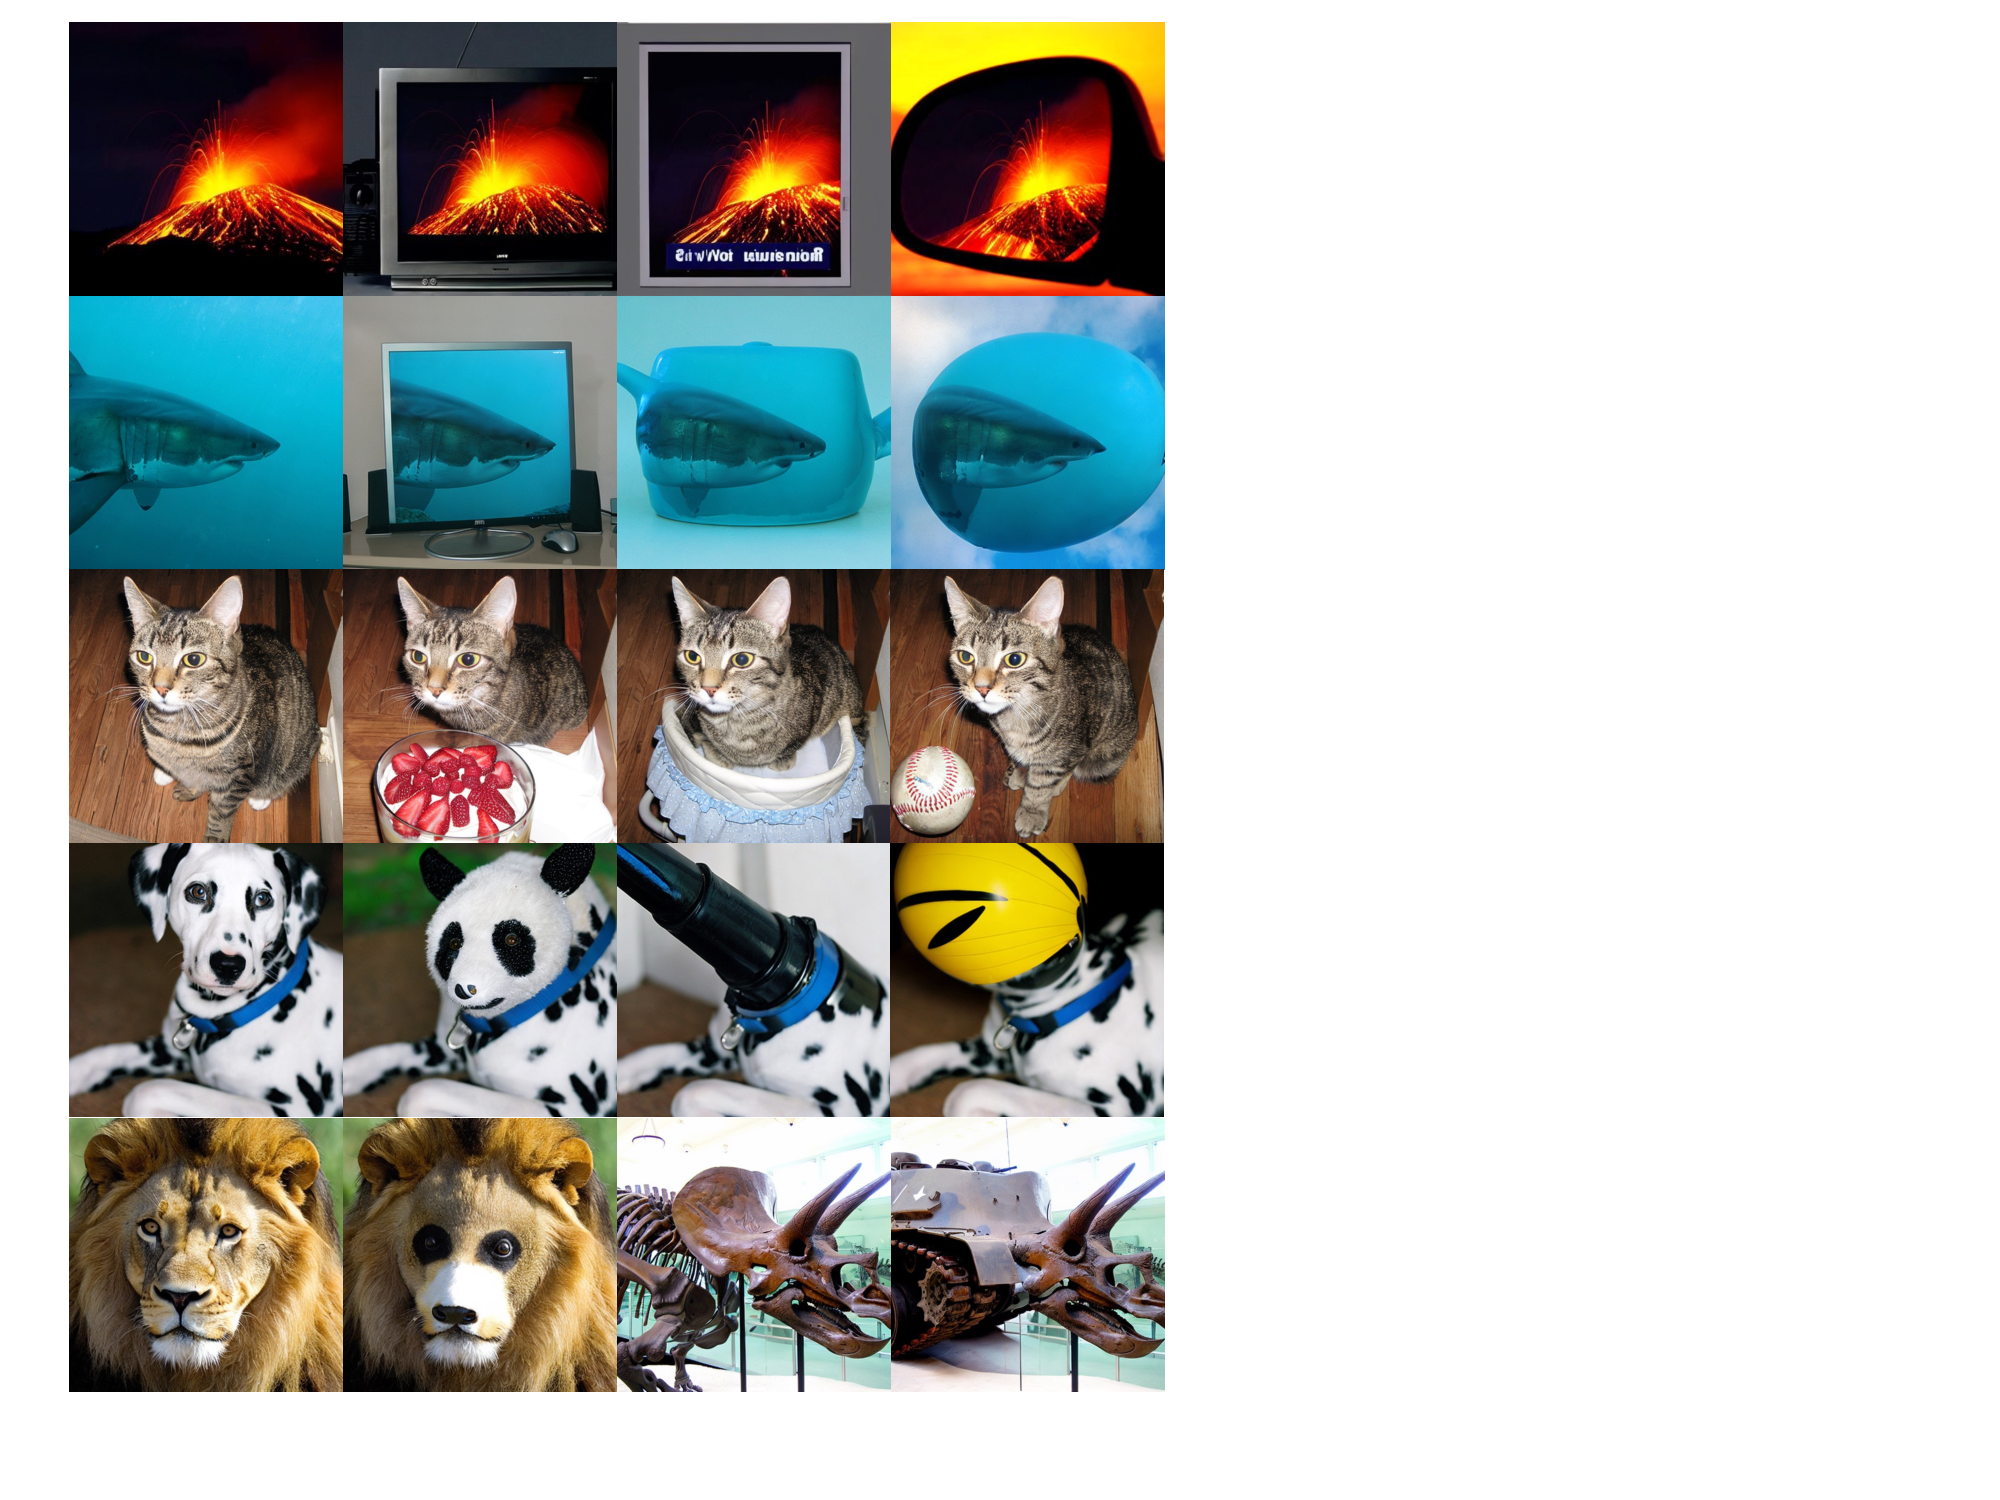
\includegraphics[width=\linewidth]{figs/edit512.pdf}
\caption{\textbf{Zero-shot editing samples.} CausalFusion-XL, resolution 512$\times$512, 800 epoch, Classifier-free guidance scale = 3.0.}
\label{fig:edit512}
\end{figure}

\begin{figure}\centering
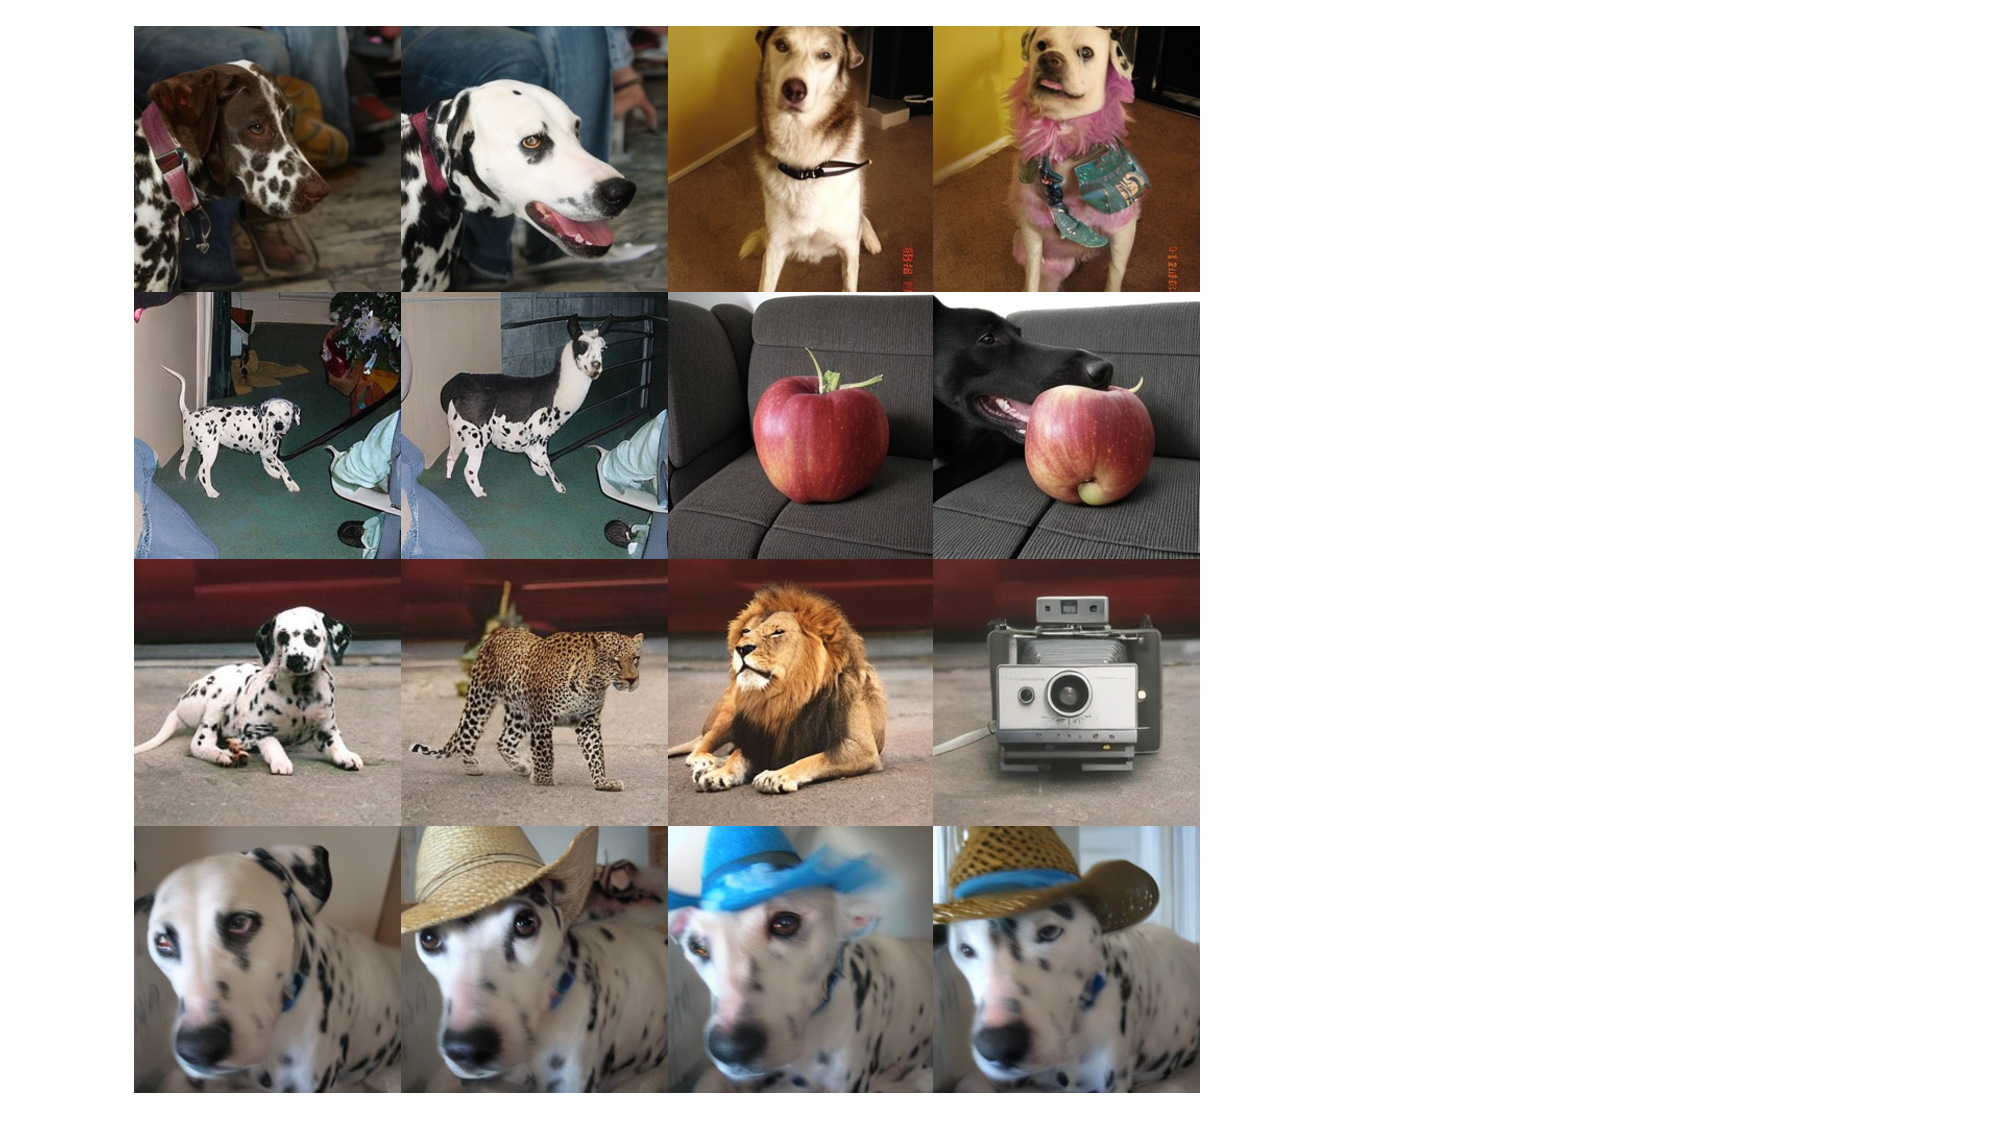
\includegraphics[width=\linewidth]{figs/edit256.pdf}
\caption{\textbf{Zero-shot editing samples.} CausalFusion-XL, resolution 256$\times$256, 800 epoch, Classifier-free guidance scale = 1.5.}
\label{fig:edit256}
\end{figure}


\clearpage
\begin{figure}\centering
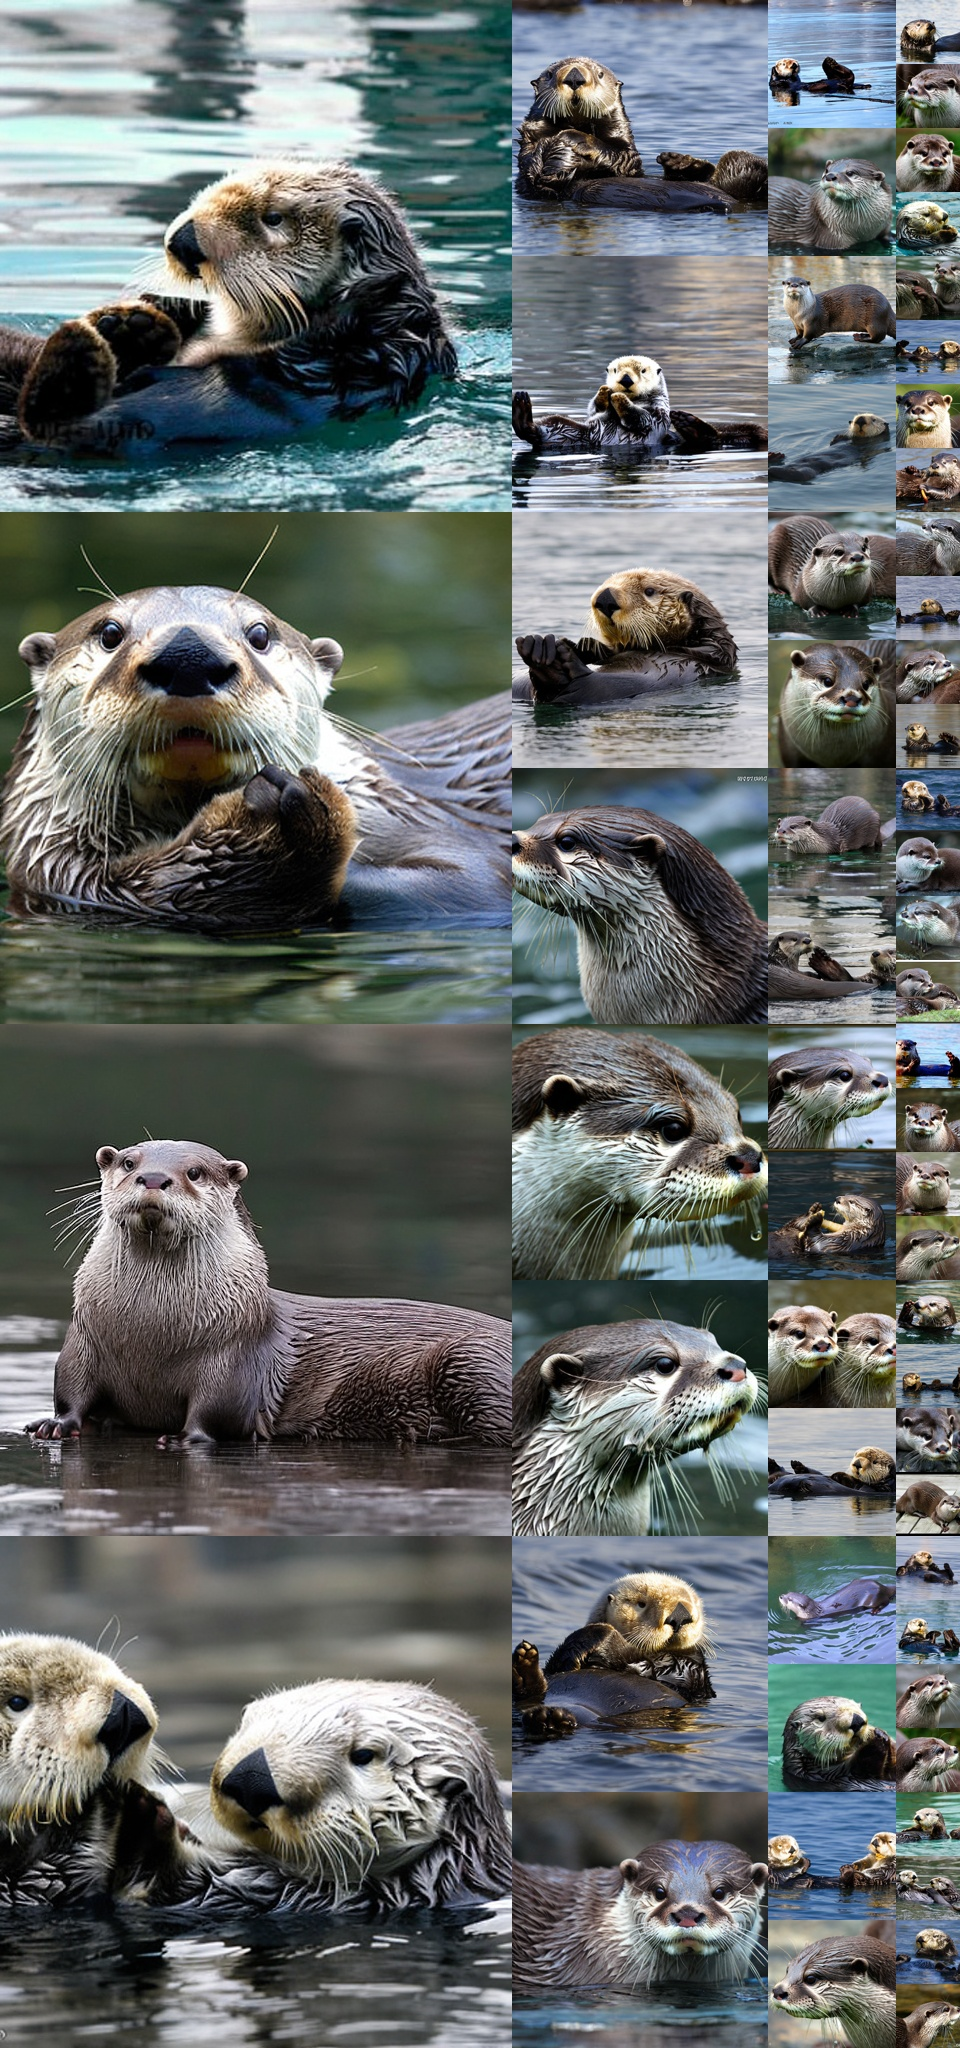
\includegraphics[width=\linewidth]{figs/xl512_360_cfg4.0.jpg}
\caption{\textbf{Uncurated $512\times512$ CausalFusion-XL samples.} \\Classifier-free guidance scale = 4.0\\Class label = ``otter" (360)}\vspace{-2mm}
\label{fig:samples512_1}
\end{figure}

\begin{figure}\centering
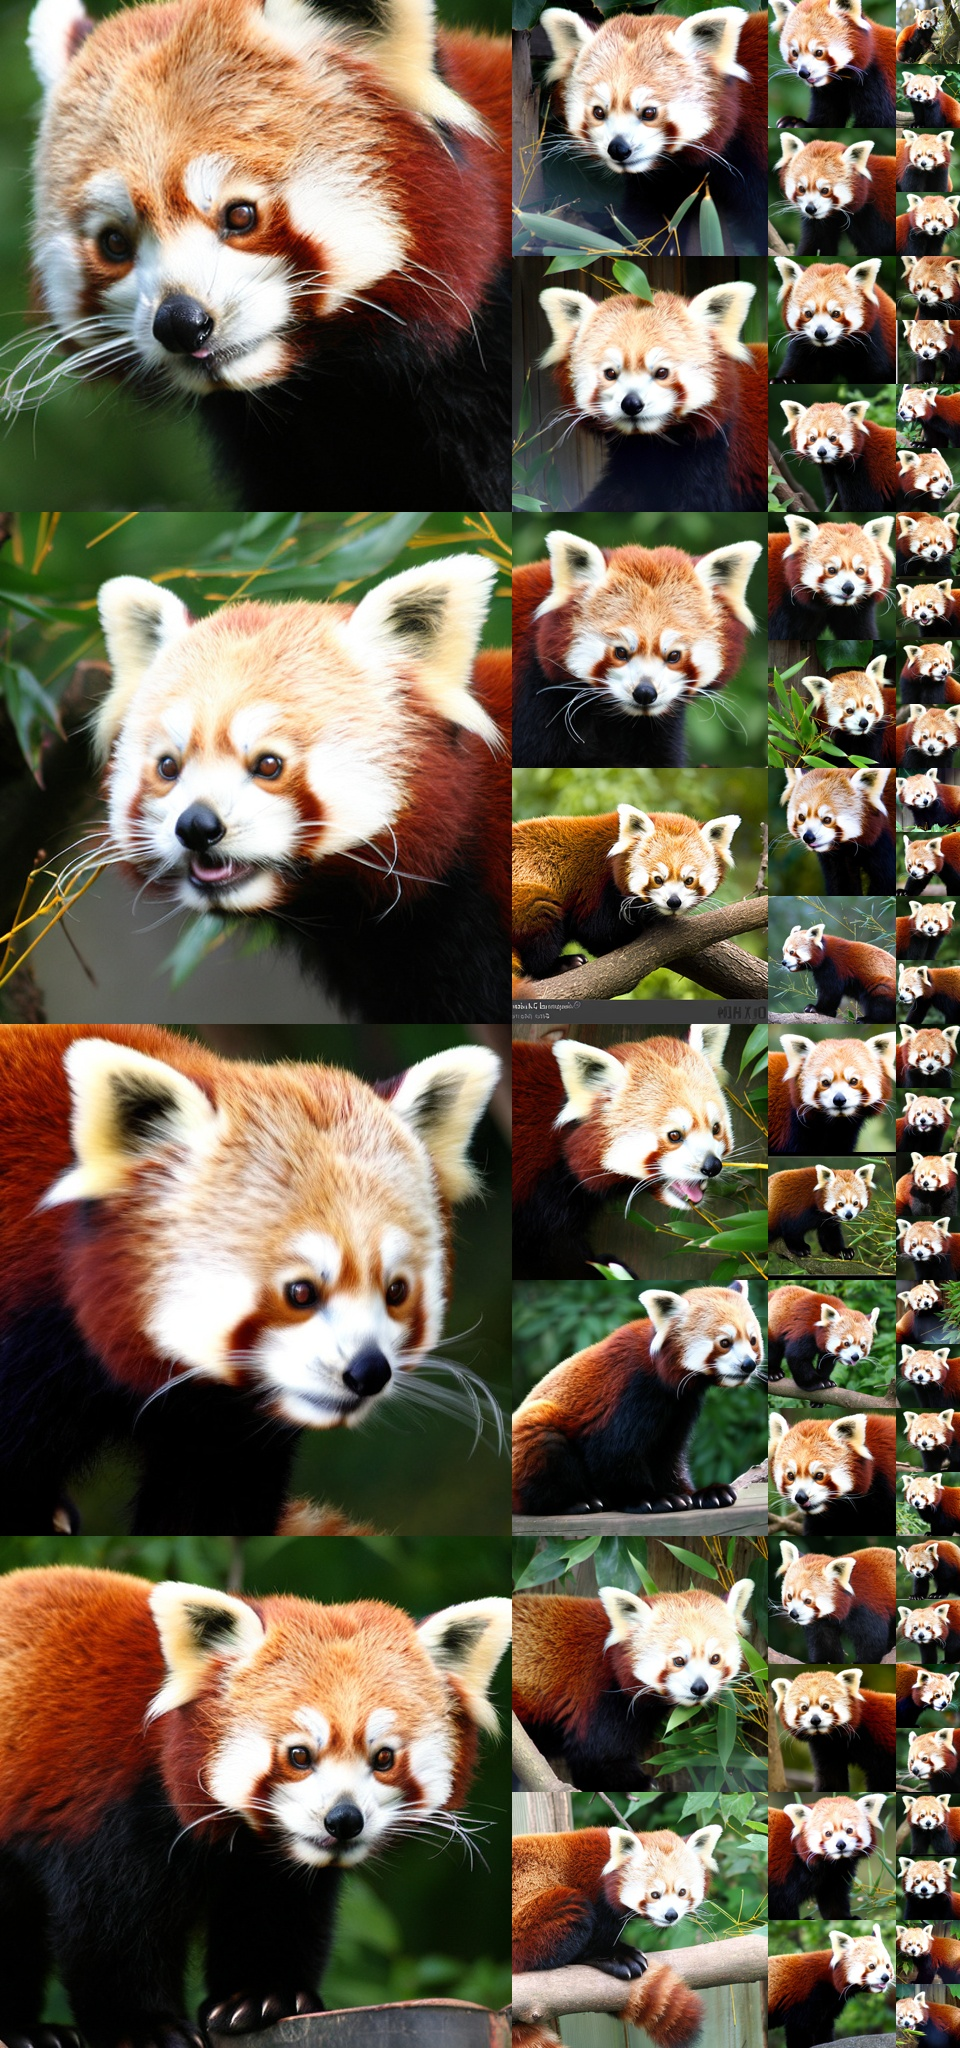
\includegraphics[width=\linewidth]{figs/xl512_387_cfg4.0.jpg}
\caption{\textbf{Uncurated $512\times512$ CausalFusion-XL samples.} \\Classifier-free guidance scale = 4.0\\Class label = ``red panda" (387)}\vspace{-2mm}
\label{fig:samples512_2}
\end{figure}

\begin{figure}\centering
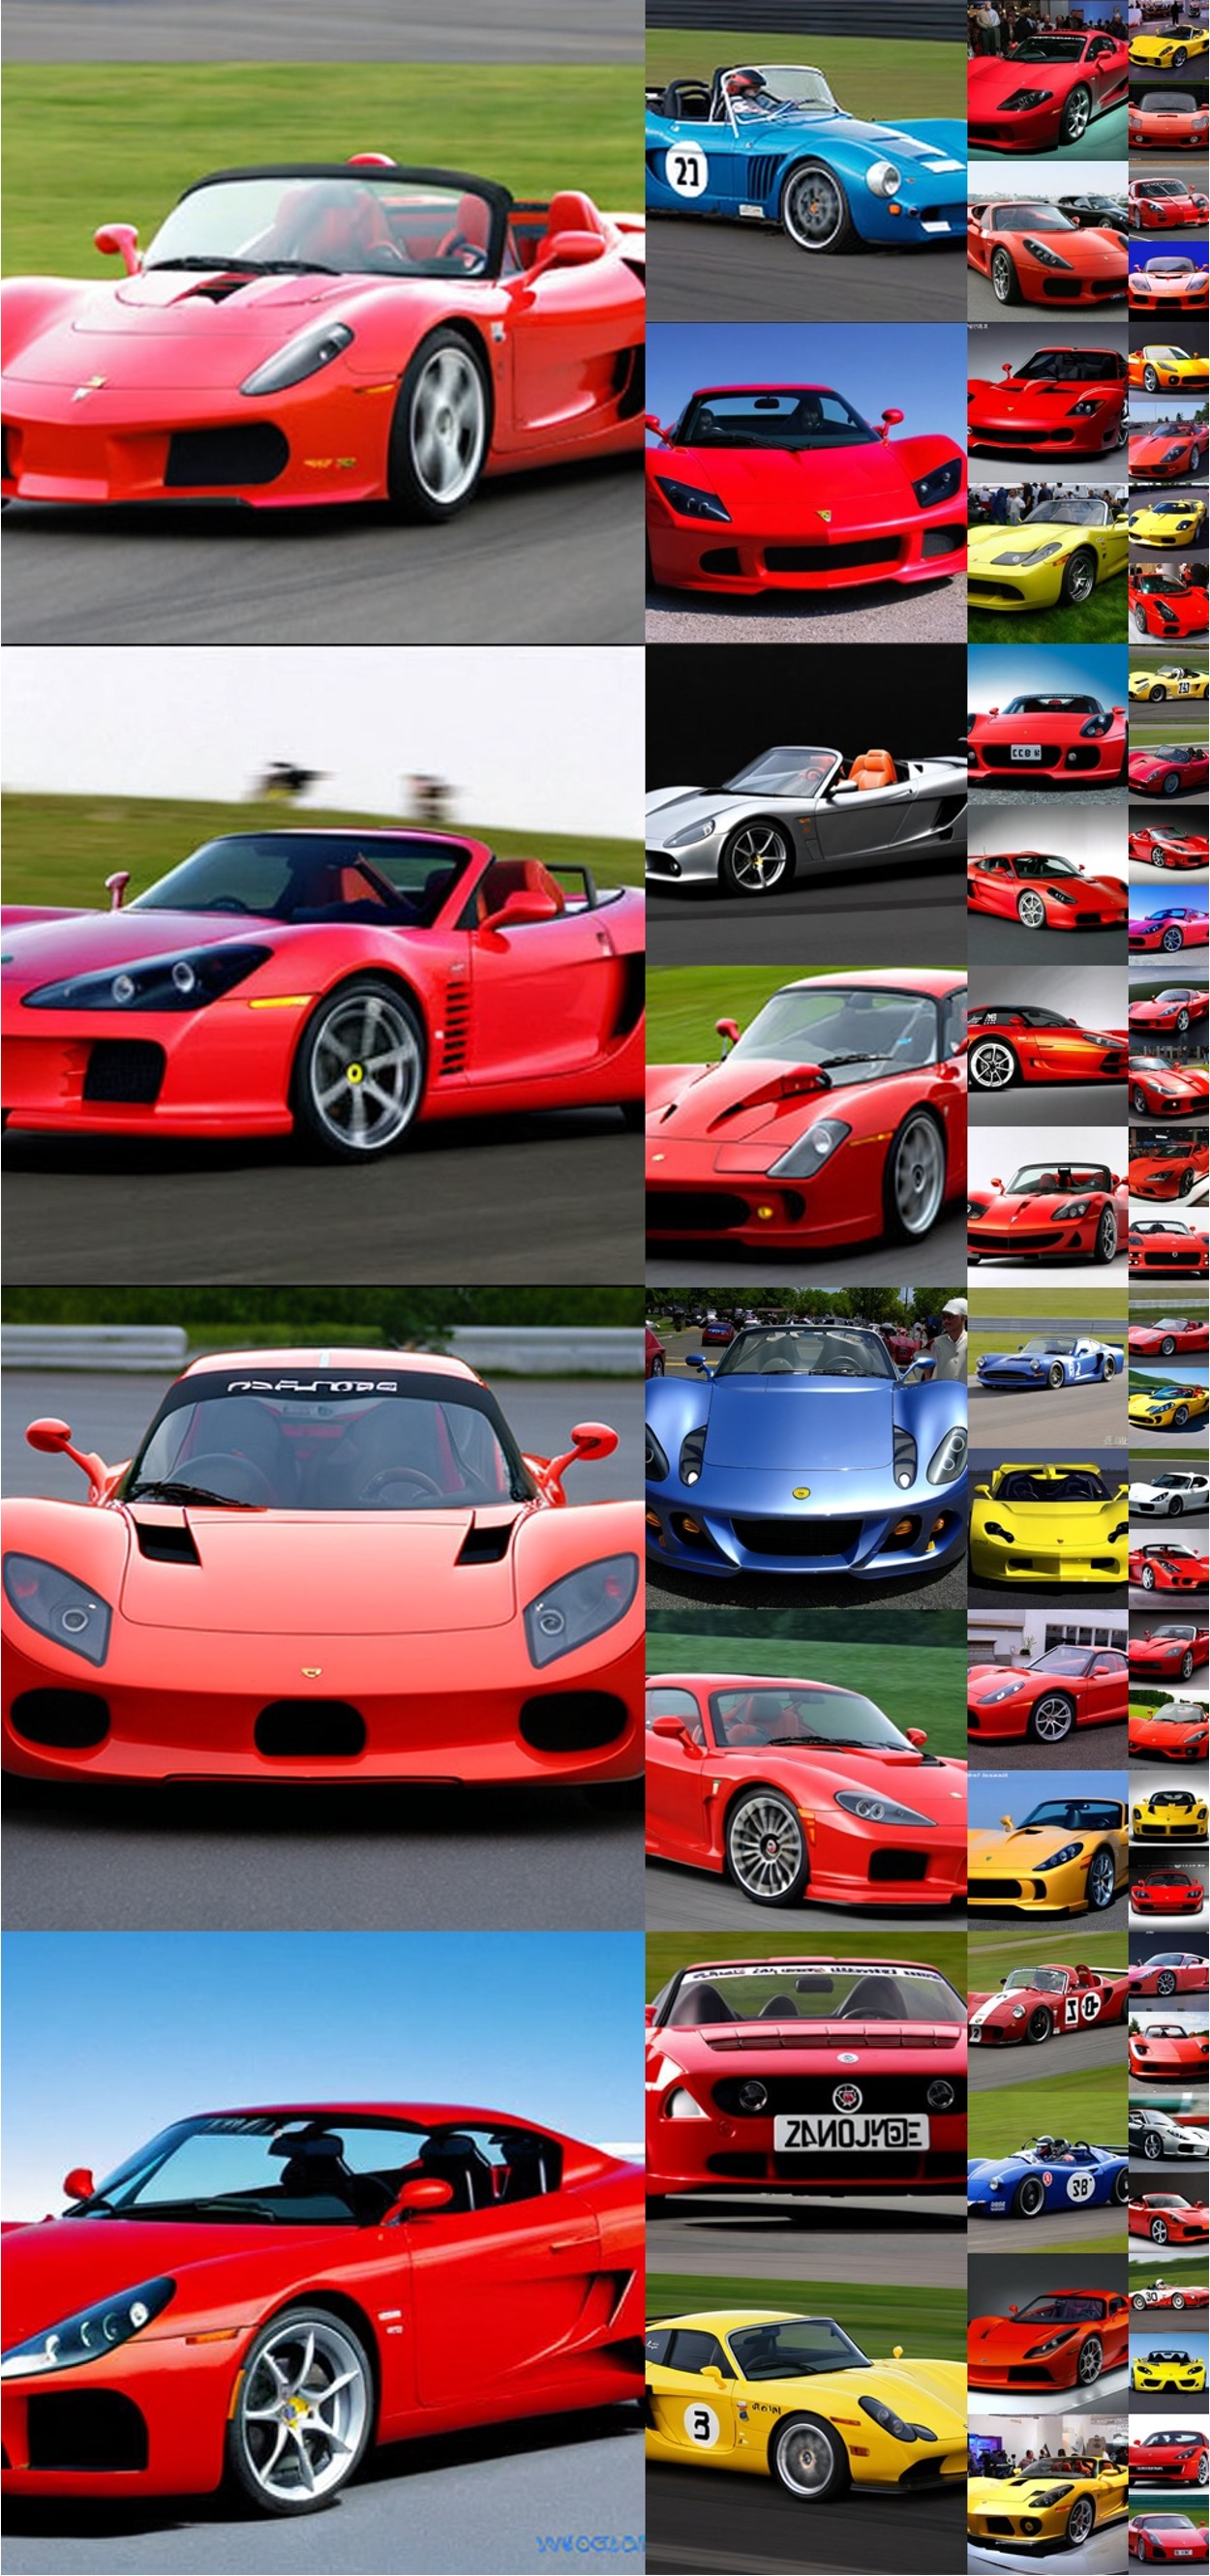
\includegraphics[width=\linewidth]{figs/xl512_817_cfg4.0.jpg}
\caption{\textbf{Uncurated $512\times512$ CausalFusion-XL samples.} \\Classifier-free guidance scale = 4.0\\Class label = ``sports car" (817)}\vspace{-2mm}
\label{fig:samples512_3}
\end{figure}

\begin{figure}\centering
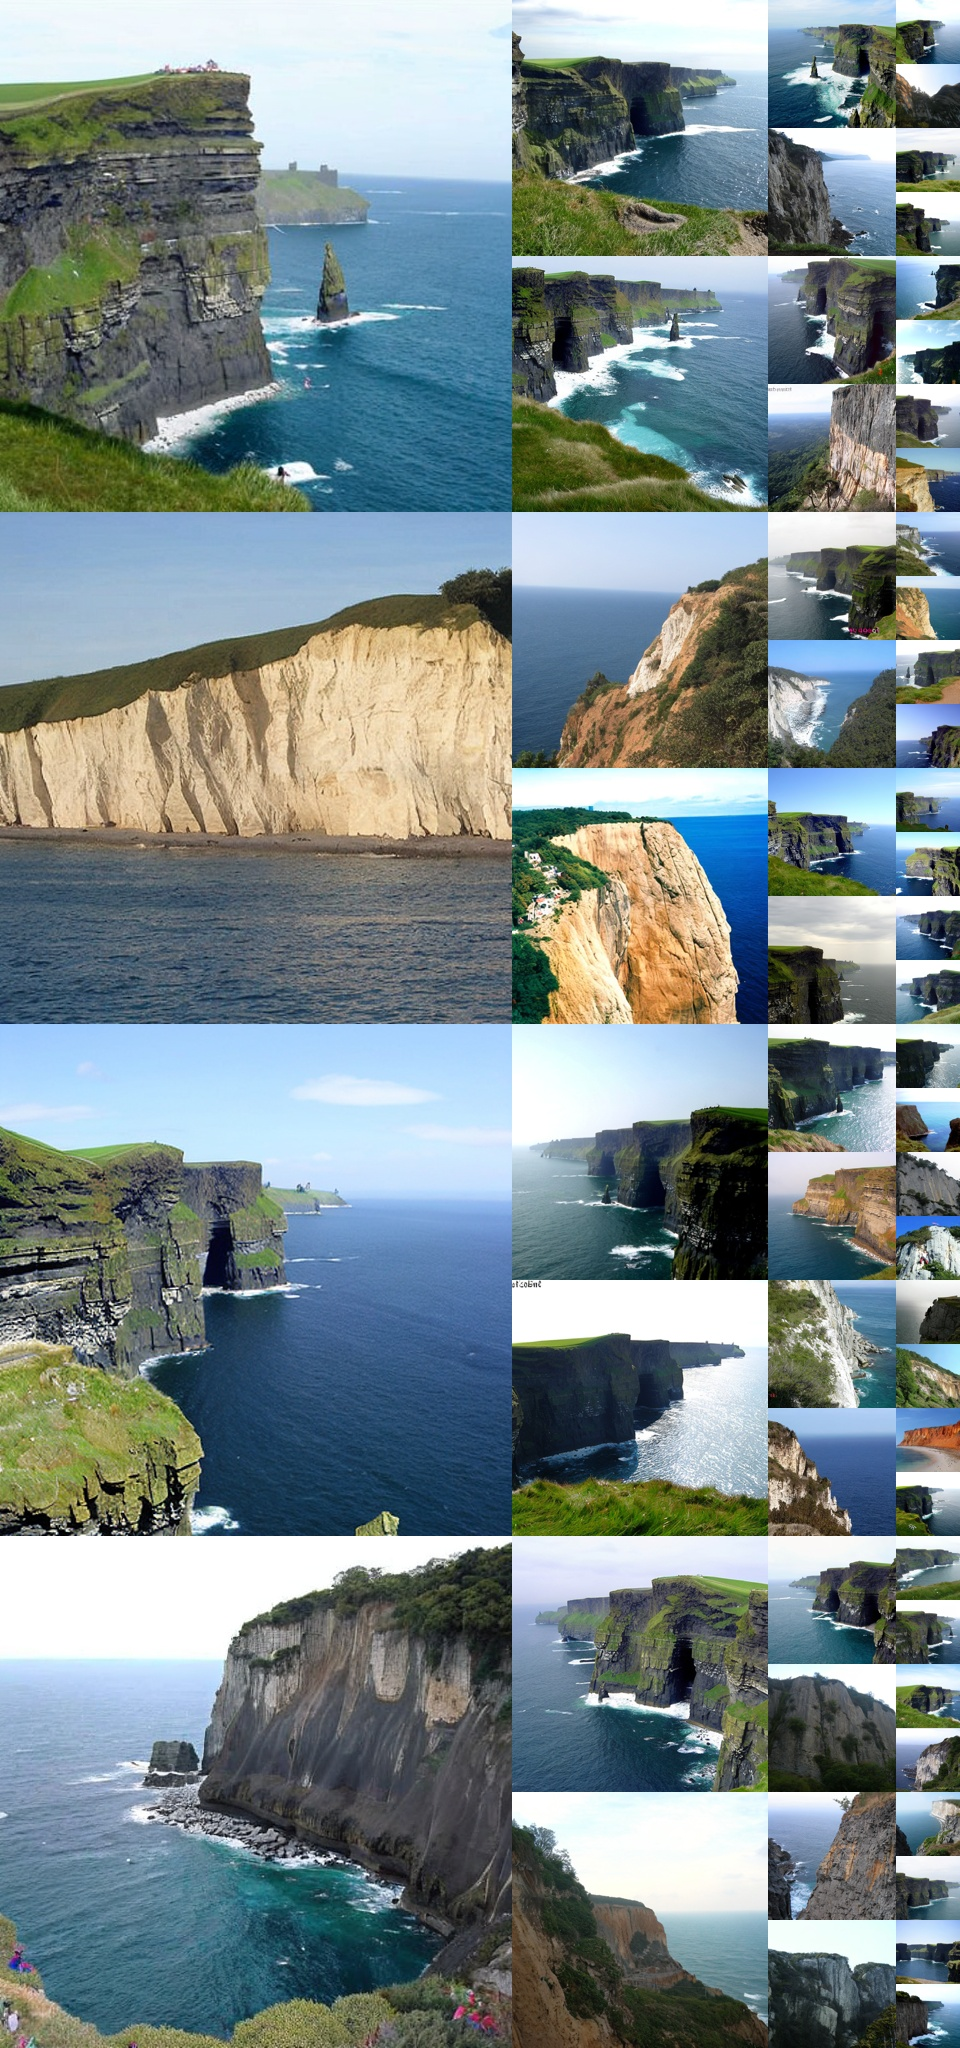
\includegraphics[width=\linewidth]{figs/xl512_972_cfg4.0.jpg}
\caption{\textbf{Uncurated $512\times512$ CausalFusion-XL samples.} \\Classifier-free guidance scale = 4.0\\Class label = ``cliff" (972)}\vspace{-2mm}
\label{fig:samples512_4}
\end{figure}

\begin{figure}\centering
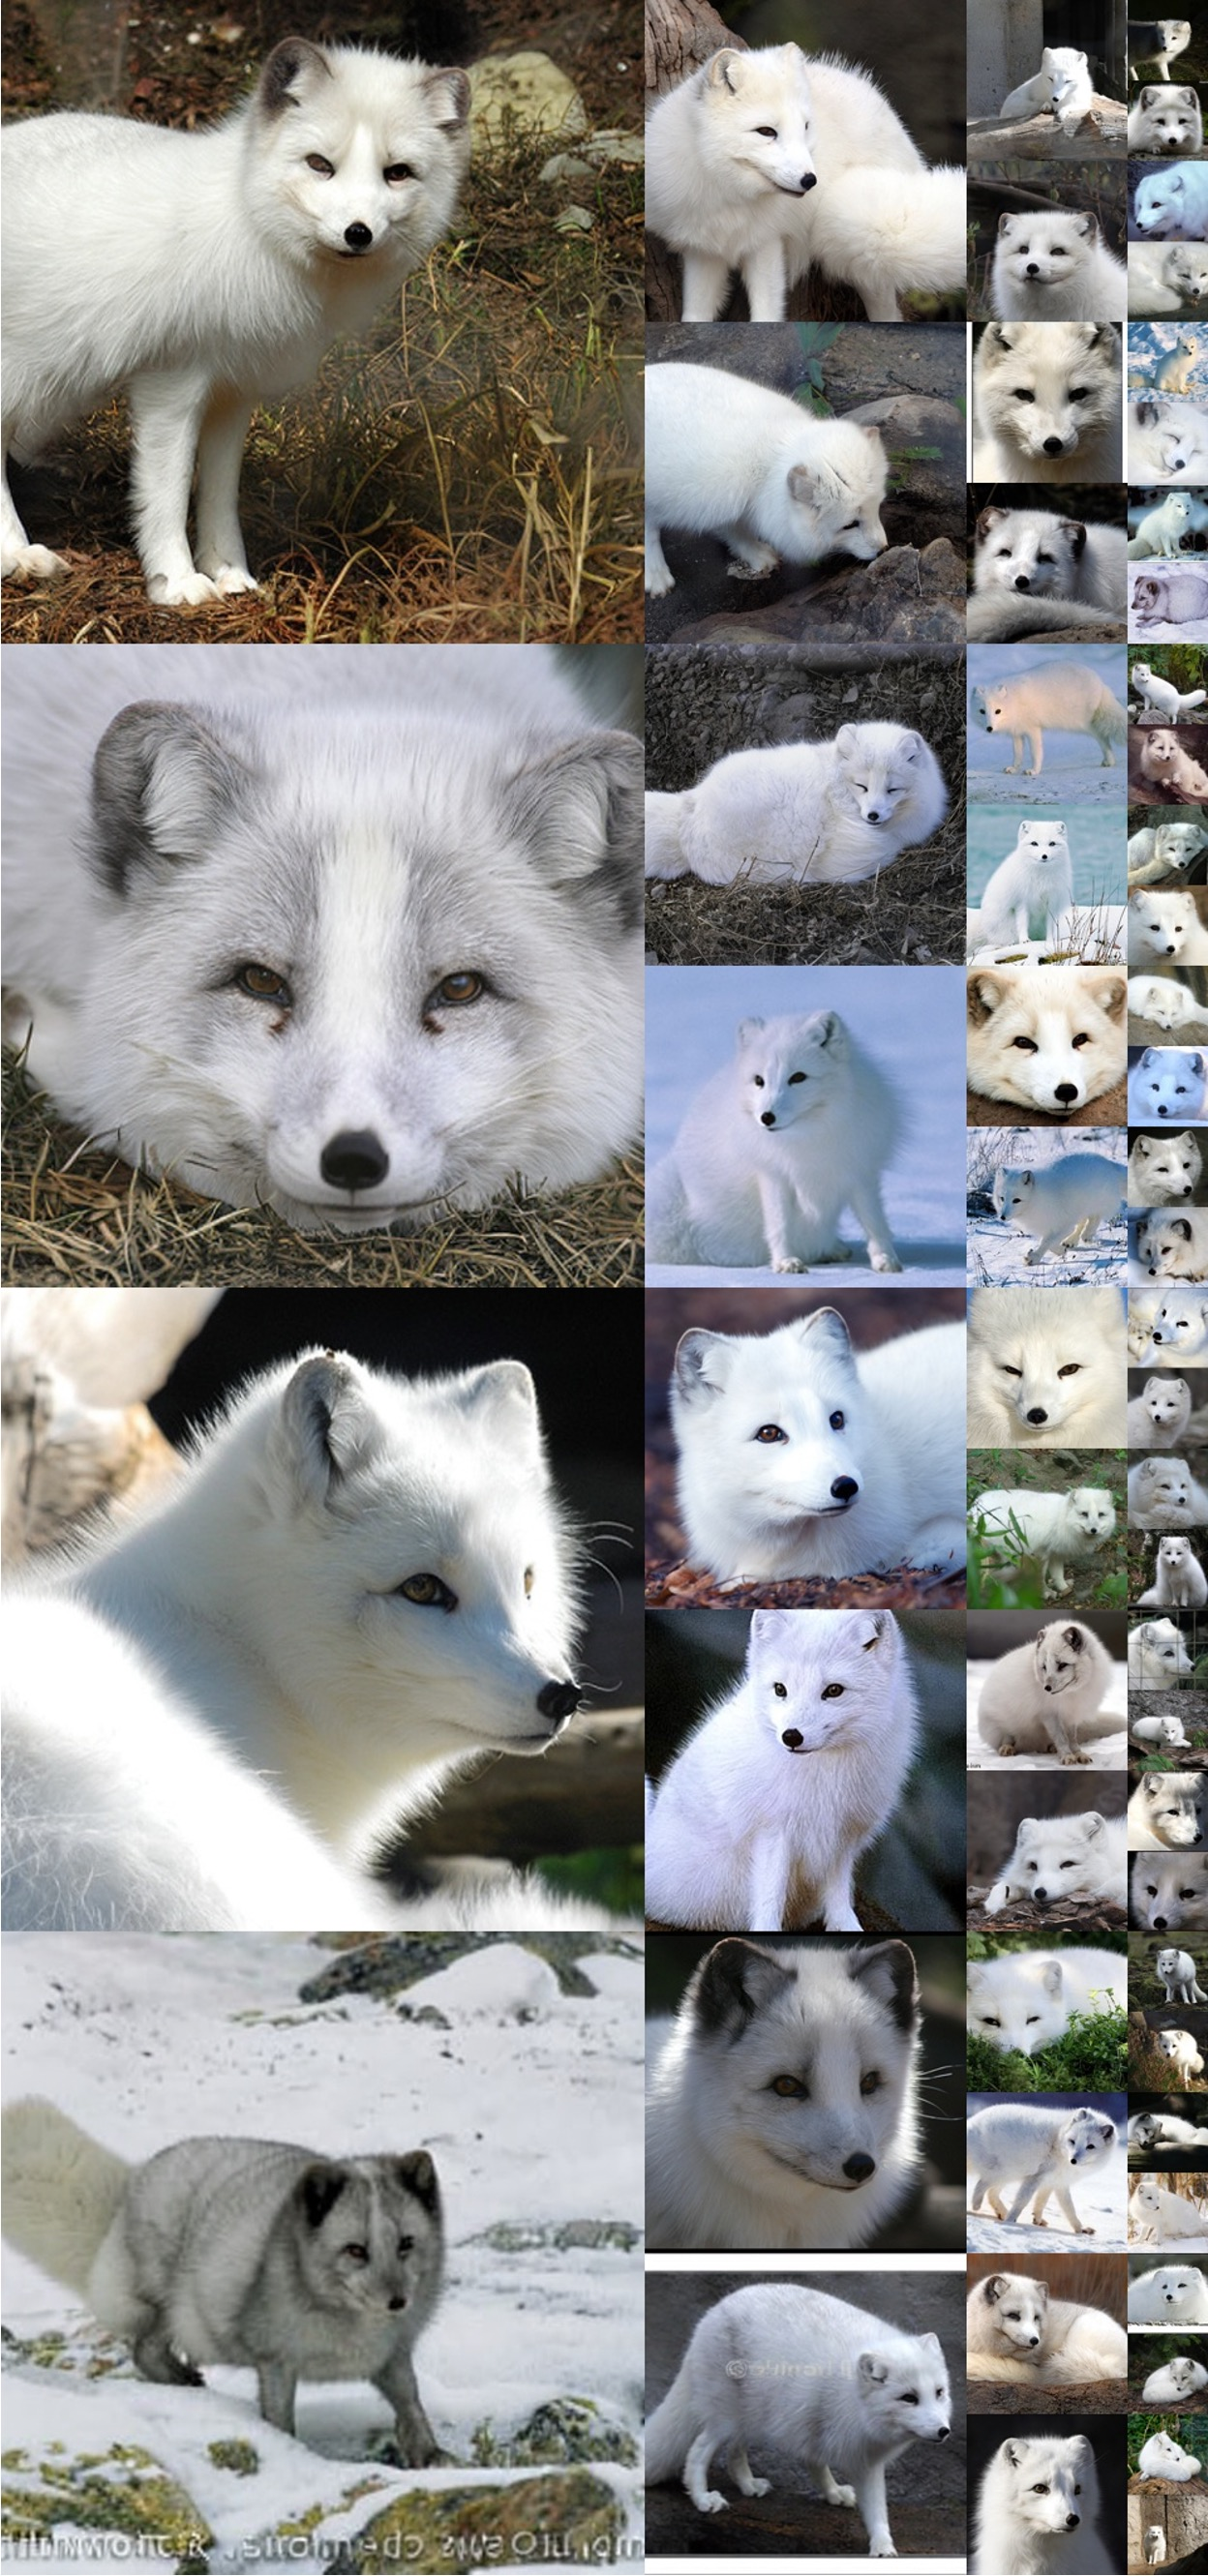
\includegraphics[width=\linewidth]{figs/xl512_279_cfg2.0.jpg}
\caption{\textbf{Uncurated $512\times512$ CausalFusion-XL samples.} \\Classifier-free guidance scale = 4.0\\Class label = ``arctic fox" (279)}\vspace{-2mm}
\label{fig:samples512_5}
\end{figure}

\begin{figure}\centering
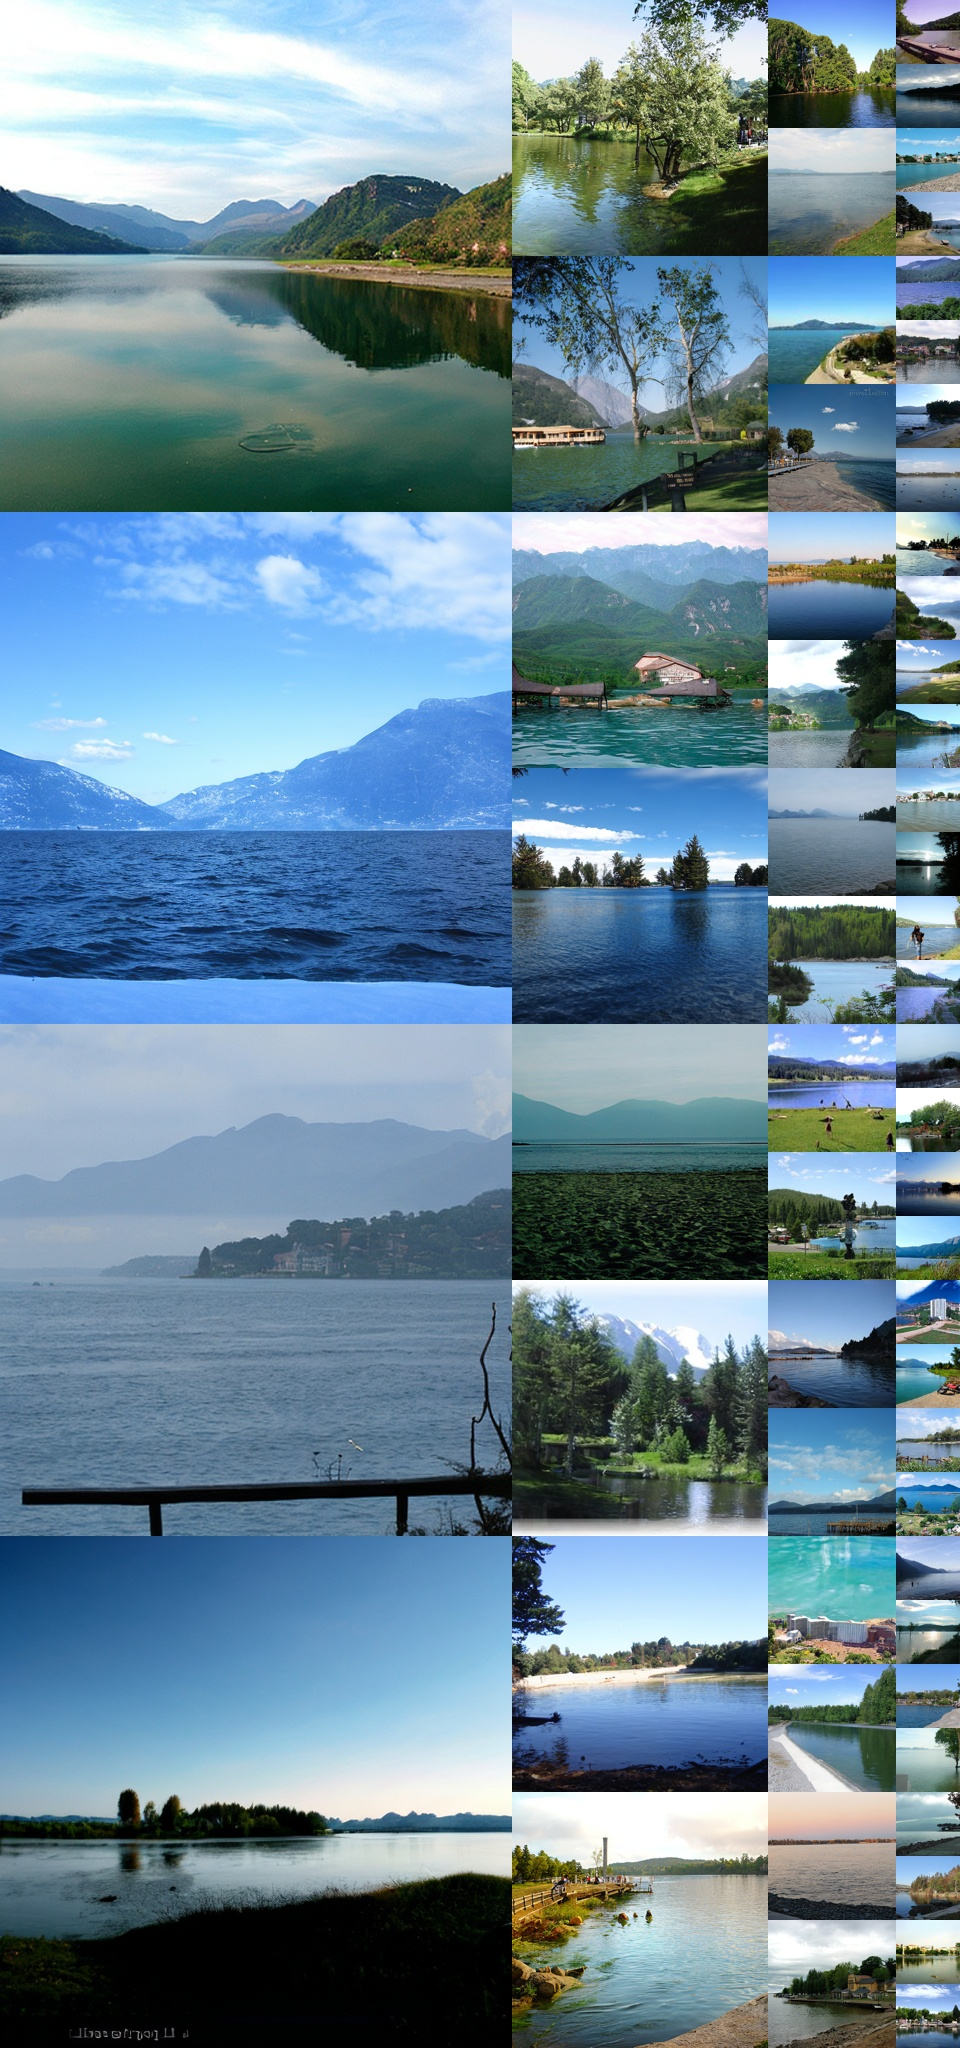
\includegraphics[width=\linewidth]{figs/xl512_975_cfg2.0.jpg}
\caption{\textbf{Uncurated $512\times512$ CausalFusion-XL samples.} \\Classifier-free guidance scale = 4.0\\Class label = ``lakeshore" (975)}\vspace{-2mm}
\label{fig:samples512_6}
\end{figure}


\begin{figure}\centering
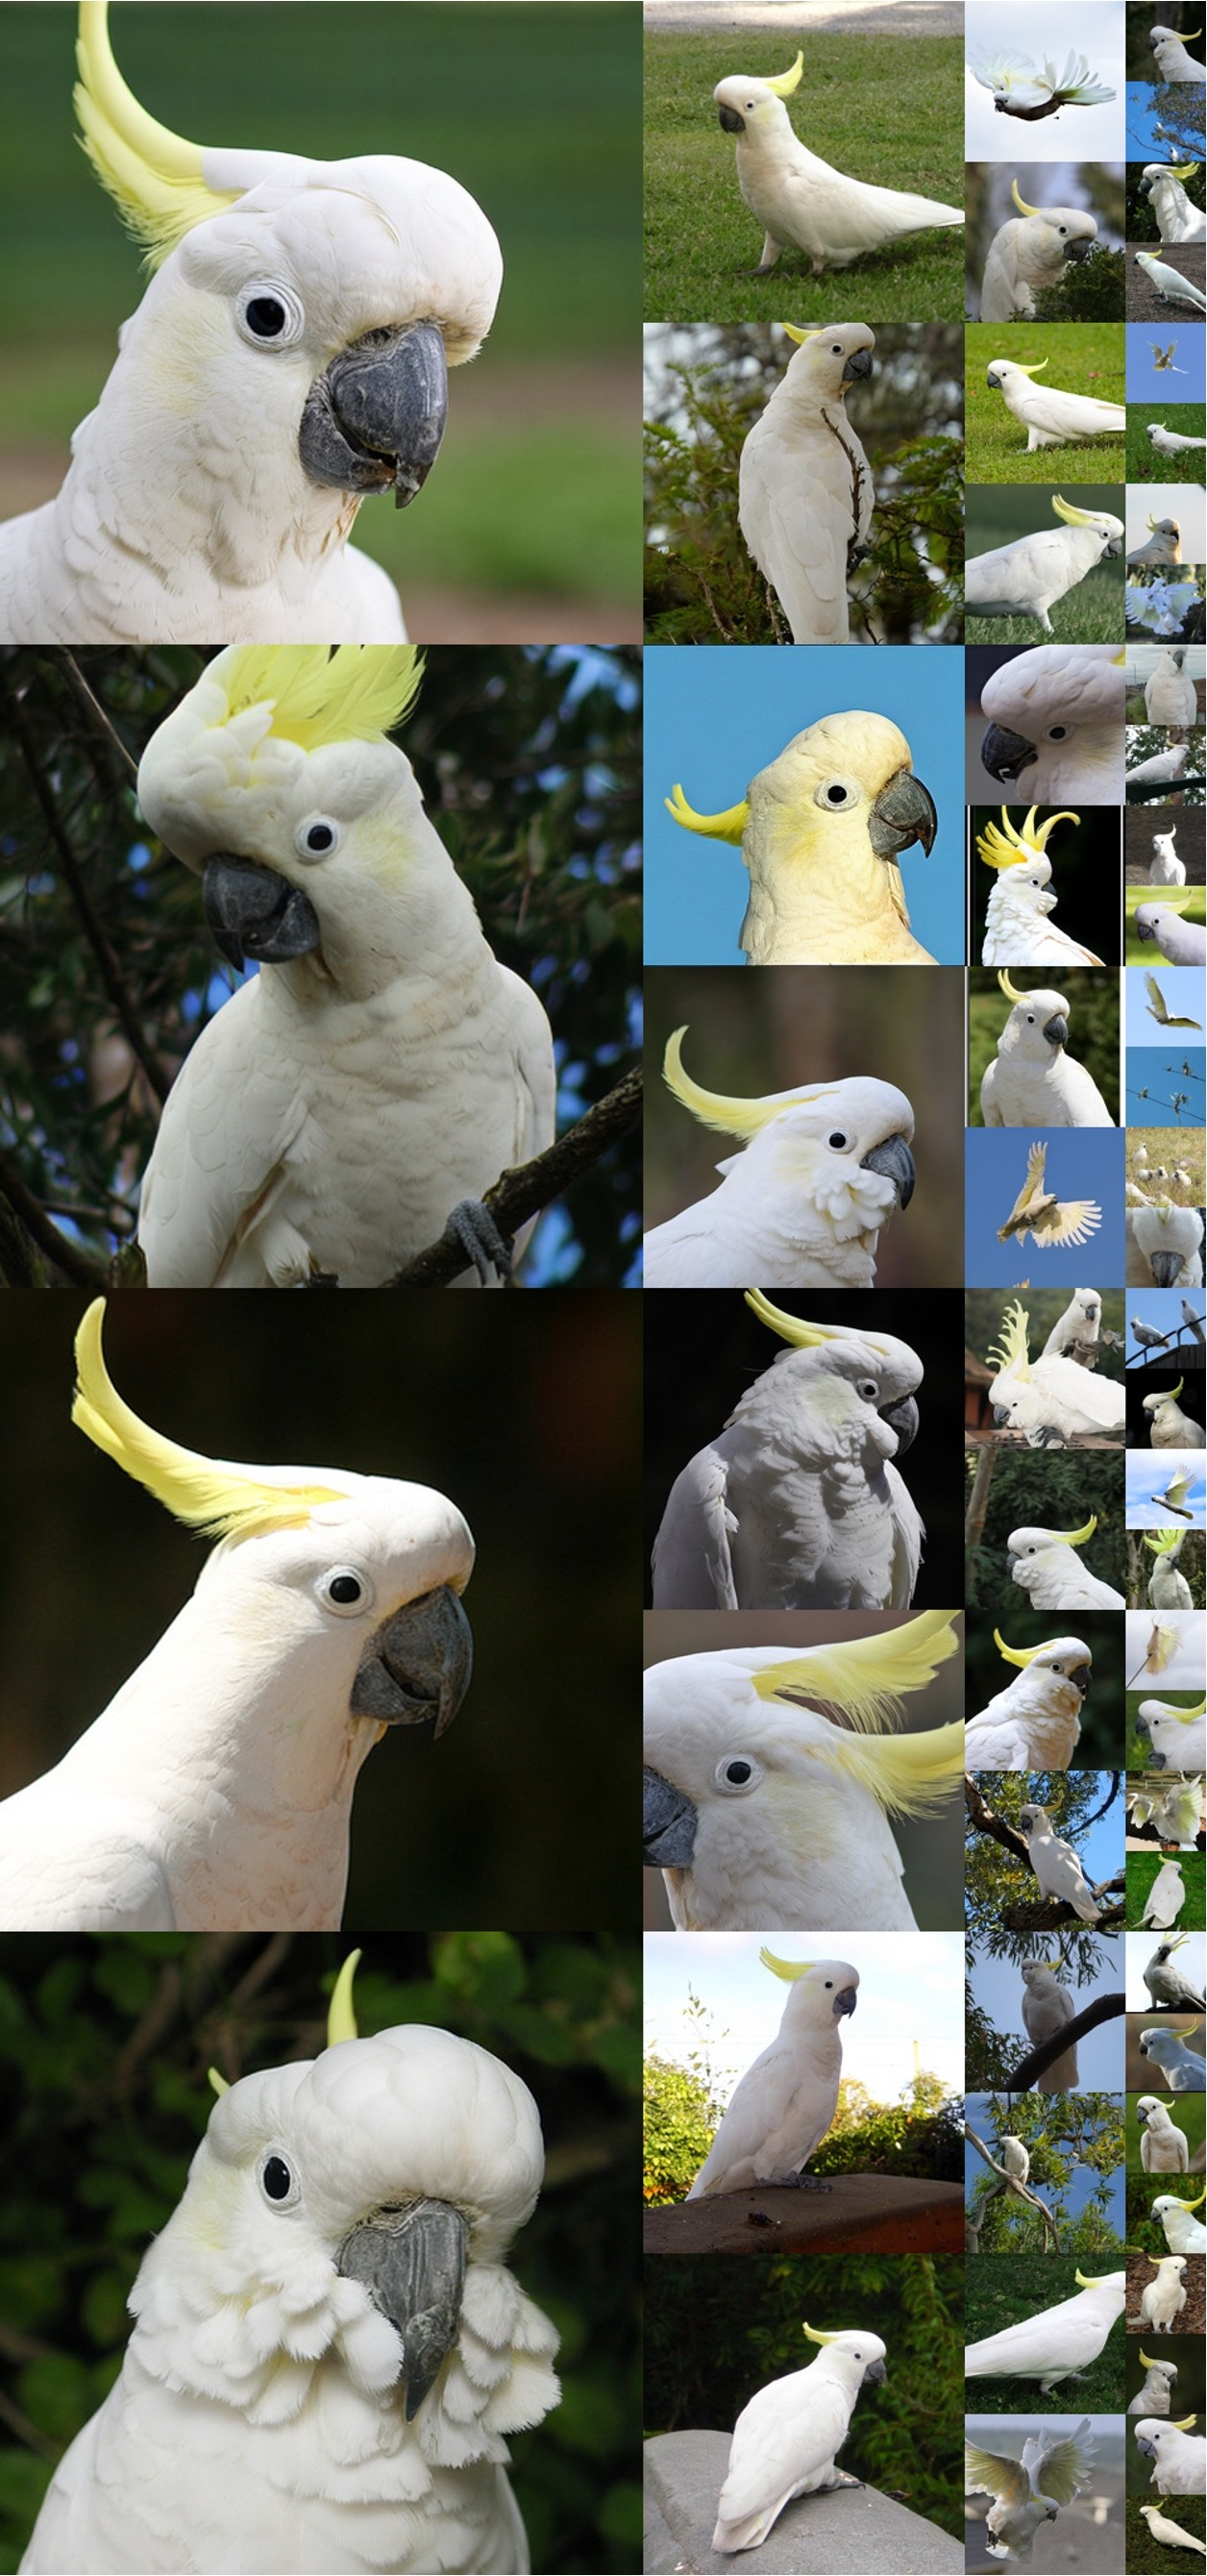
\includegraphics[width=\linewidth]{figs/xl512_89_cfg1.5.jpg}
\caption{\textbf{Uncurated $512\times512$ CausalFusion-XL samples.} \\Classifier-free guidance scale = 4.0\\Class label = ``sulphur-crested cockatoo" (89)}\vspace{-2mm}
\label{fig:samples512_7}
\end{figure}

\begin{figure}\centering
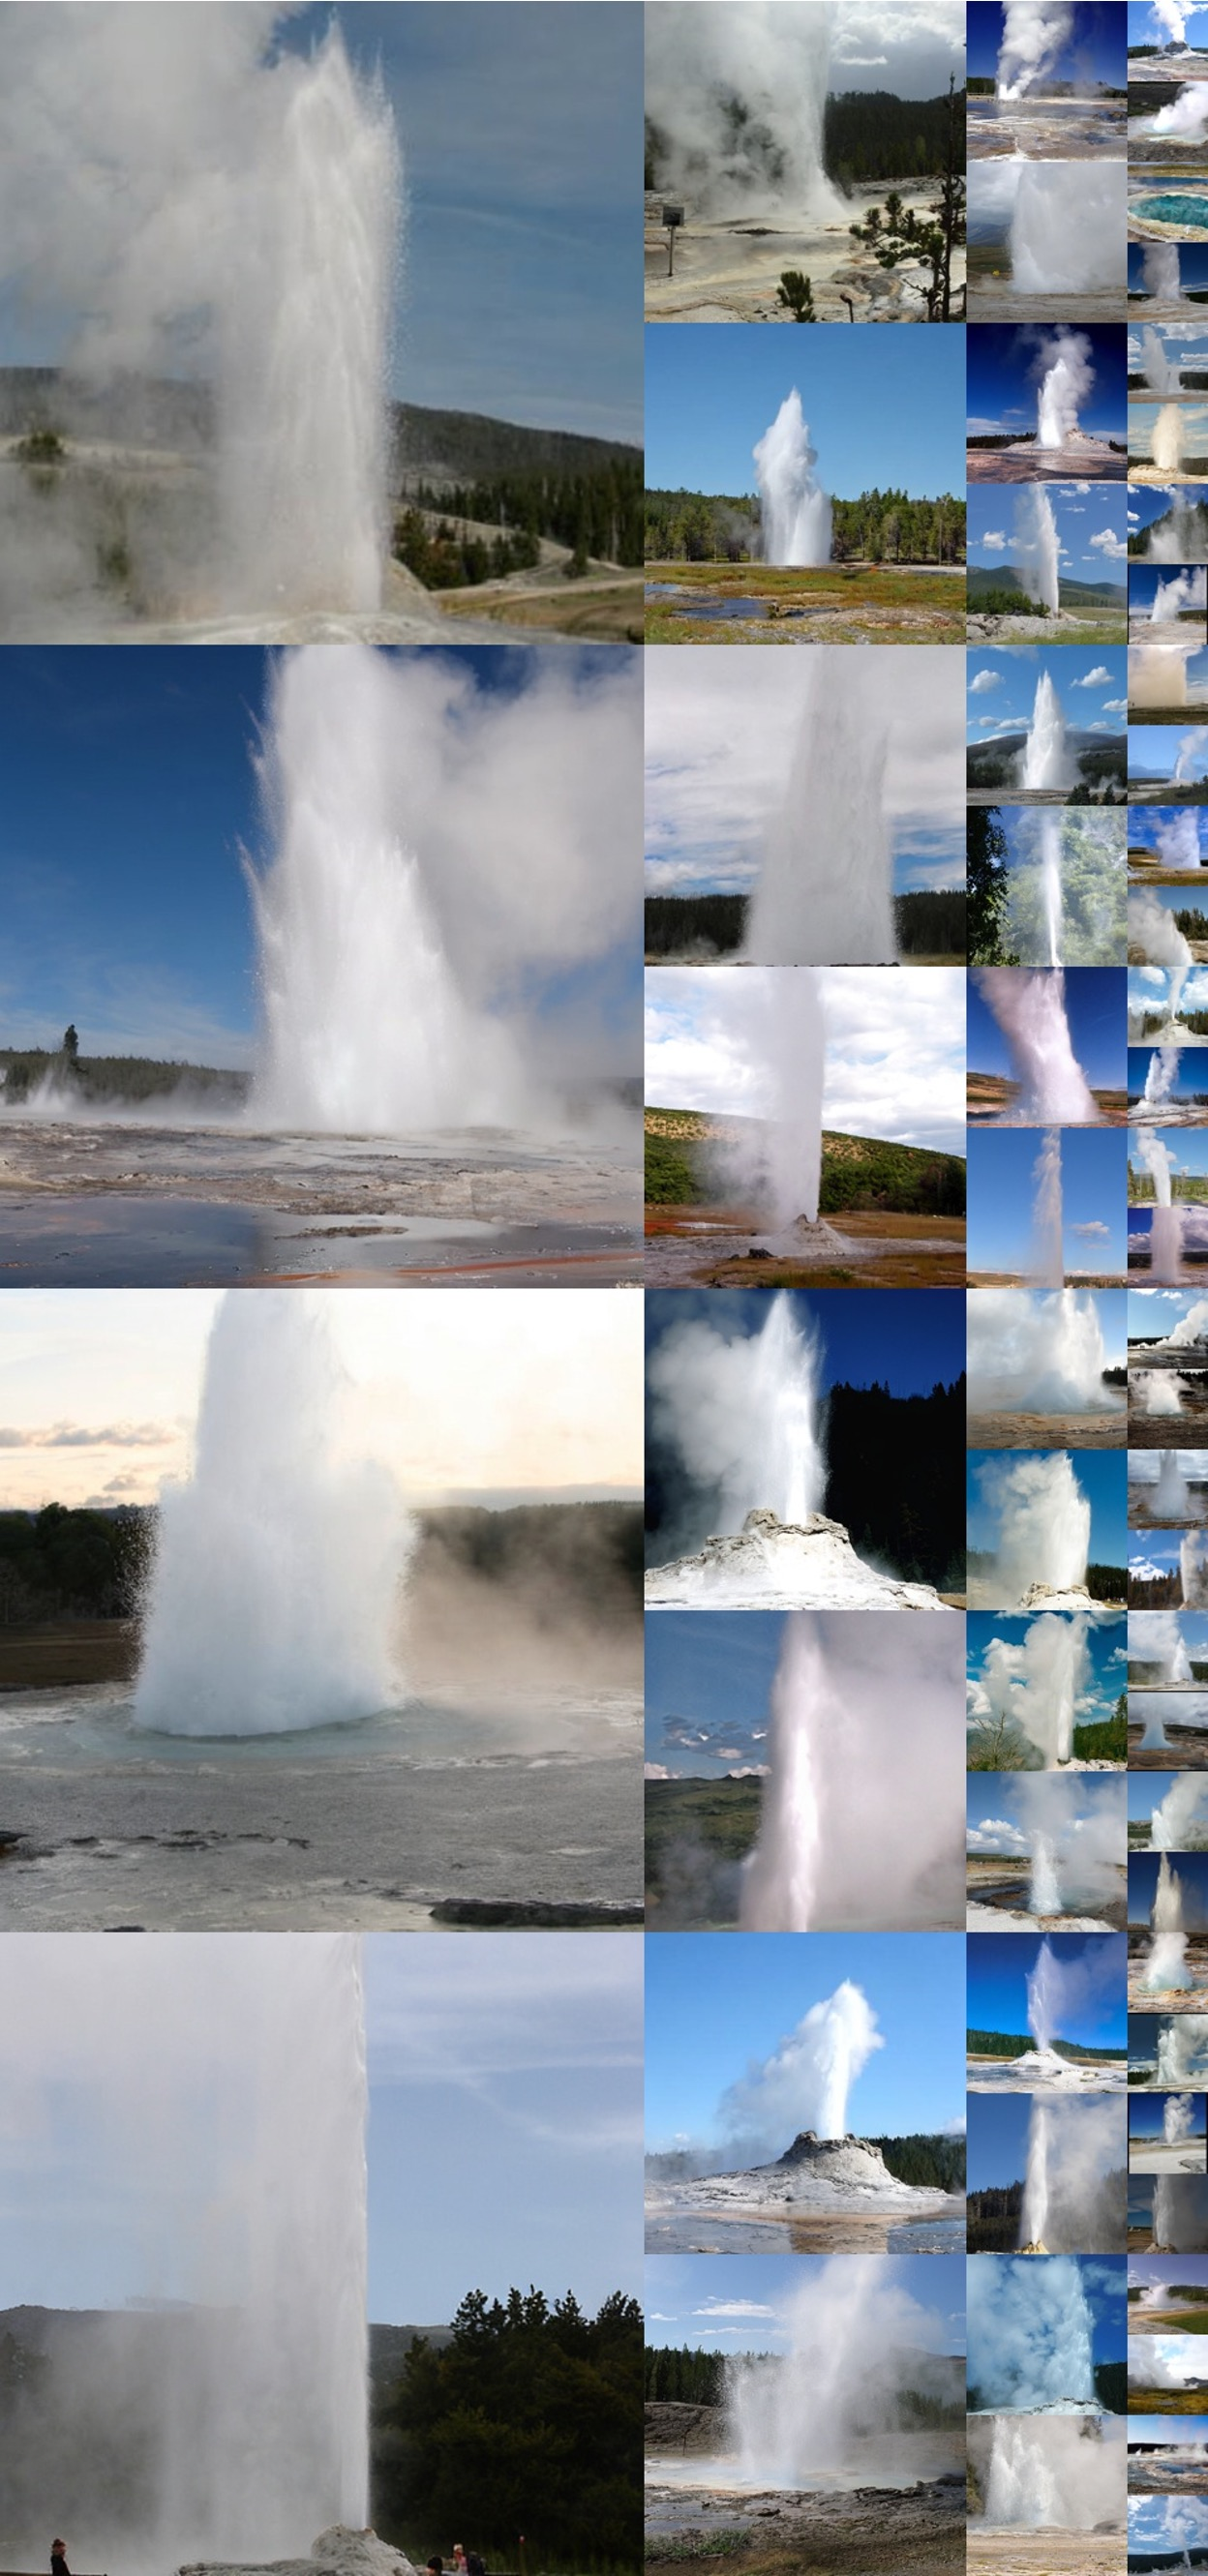
\includegraphics[width=\linewidth]{figs/xl512_974_cfg1.5.jpg}
\caption{\textbf{Uncurated $512\times512$ CausalFusion-XL samples.} \\Classifier-free guidance scale = 4.0\\Class label = ``geyser" (974)}\vspace{-2mm}
\label{fig:samples512_8}
\end{figure}


\begin{figure}\centering
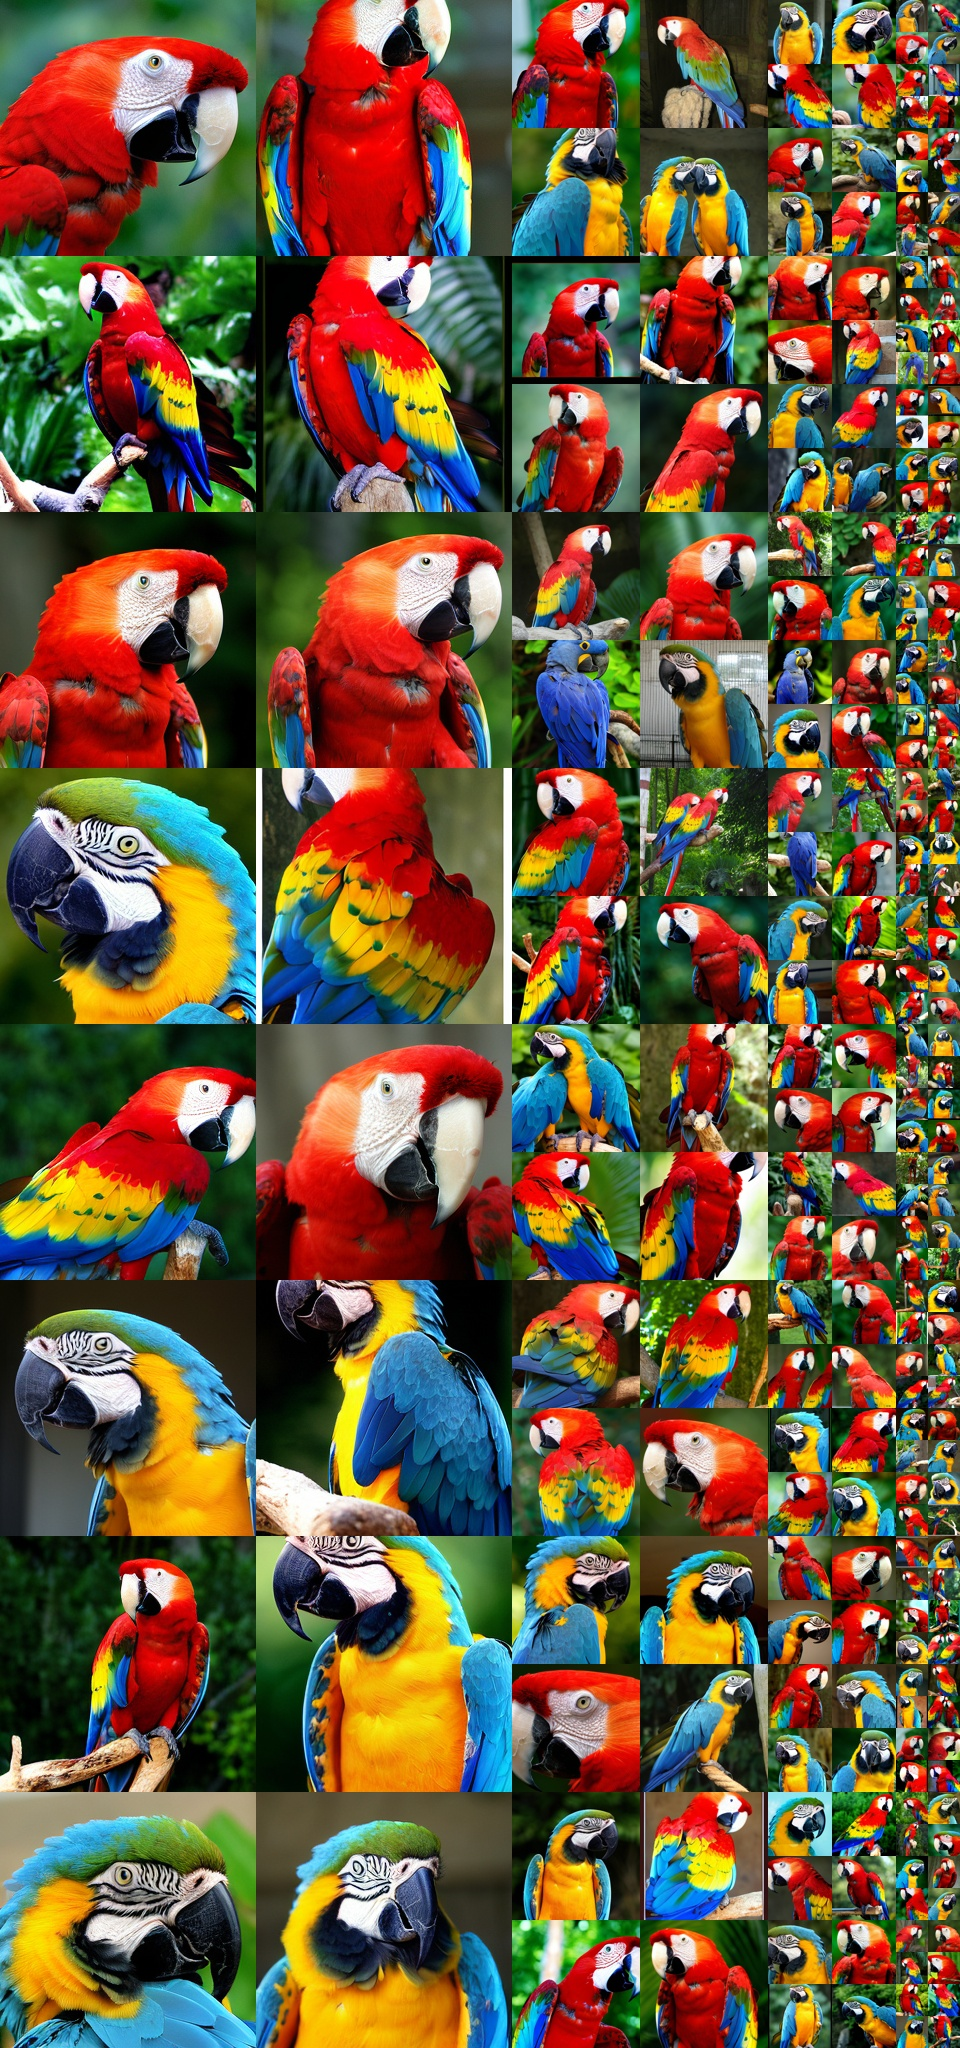
\includegraphics[width=\linewidth]{figs/xl256_88_cfg4.0.jpg}
\caption{\textbf{Uncurated $256\times256$ CausalFusion-XL samples.} \\Classifier-free guidance scale = 4.0\\Class label = ``macaw" (88)}\vspace{-2mm}
\label{fig:samples256_1}
\end{figure}

\begin{figure}\centering
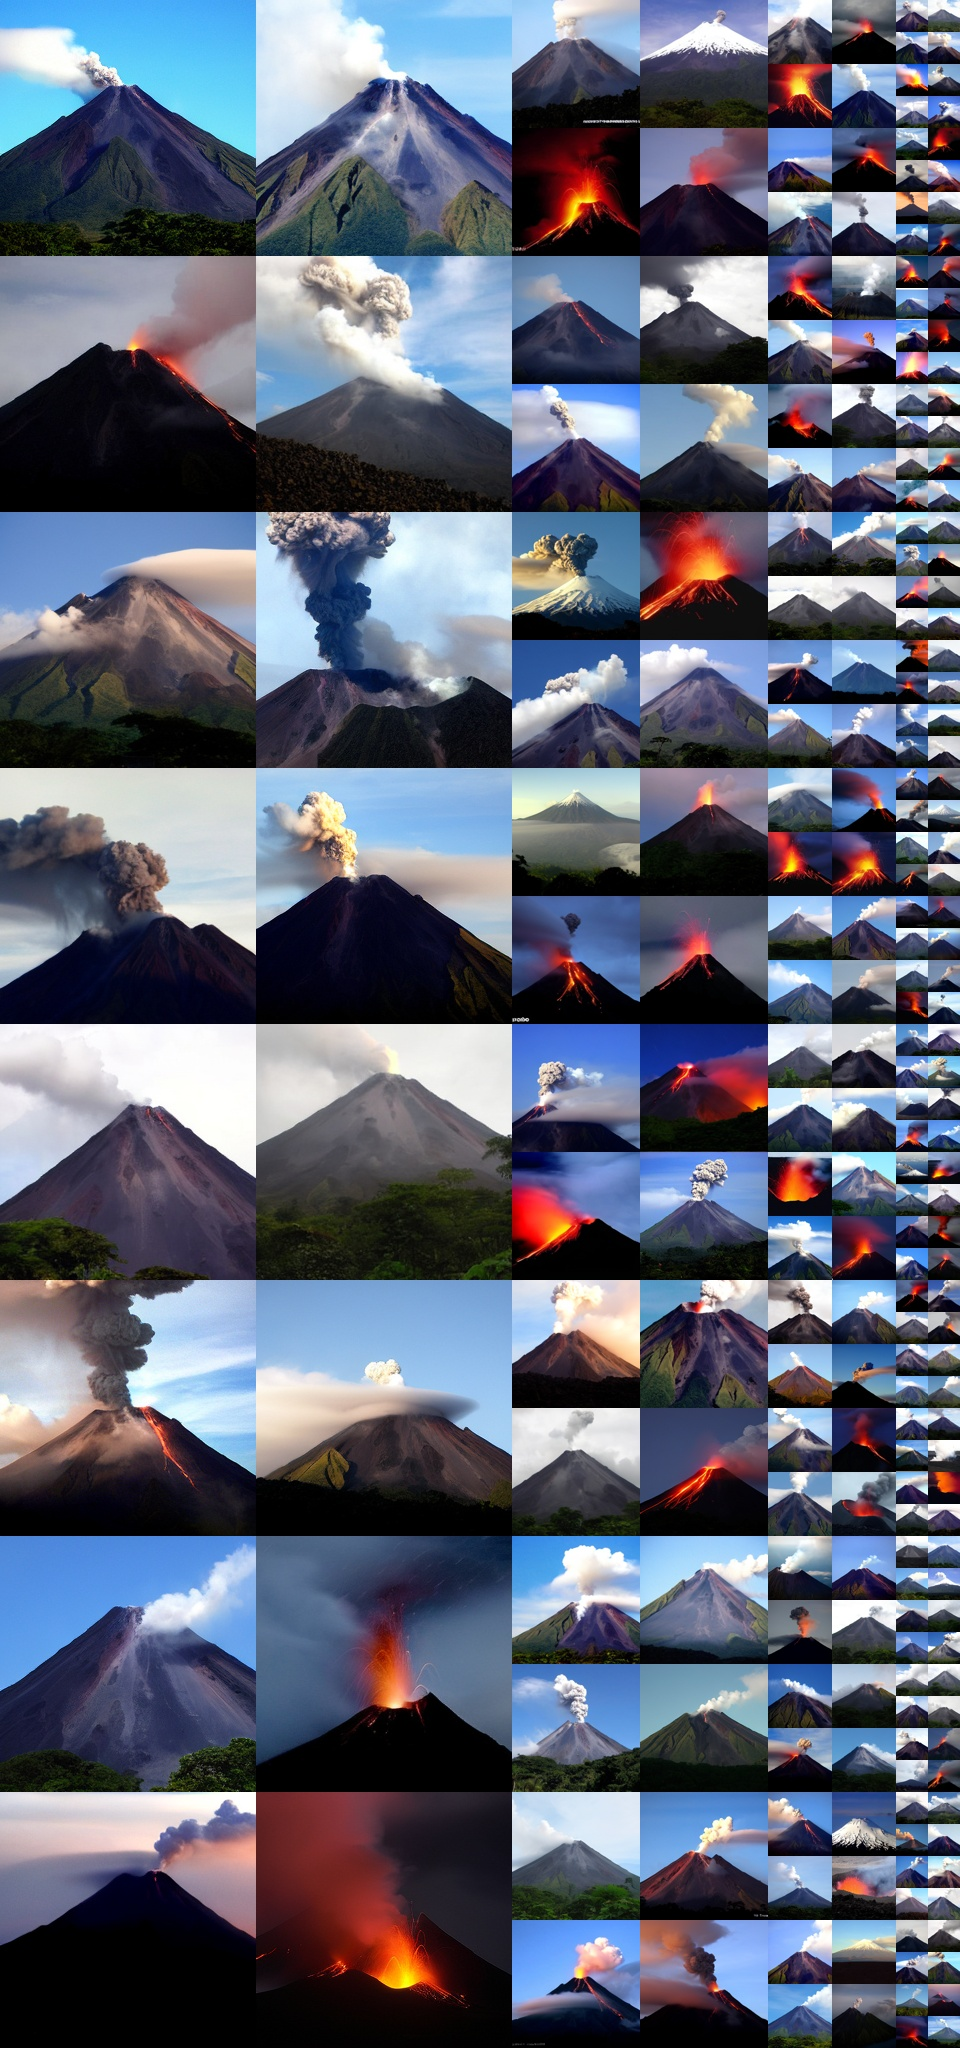
\includegraphics[width=\linewidth]{figs/xl256_980_cfg4.0.jpg}
\caption{\textbf{Uncurated $256\times256$ CausalFusion-XL samples.} \\Classifier-free guidance scale = 4.0\\Class label = ``volcano" (980)}\vspace{-2mm}
\label{fig:samples256_2}
\end{figure}


\begin{figure}\centering
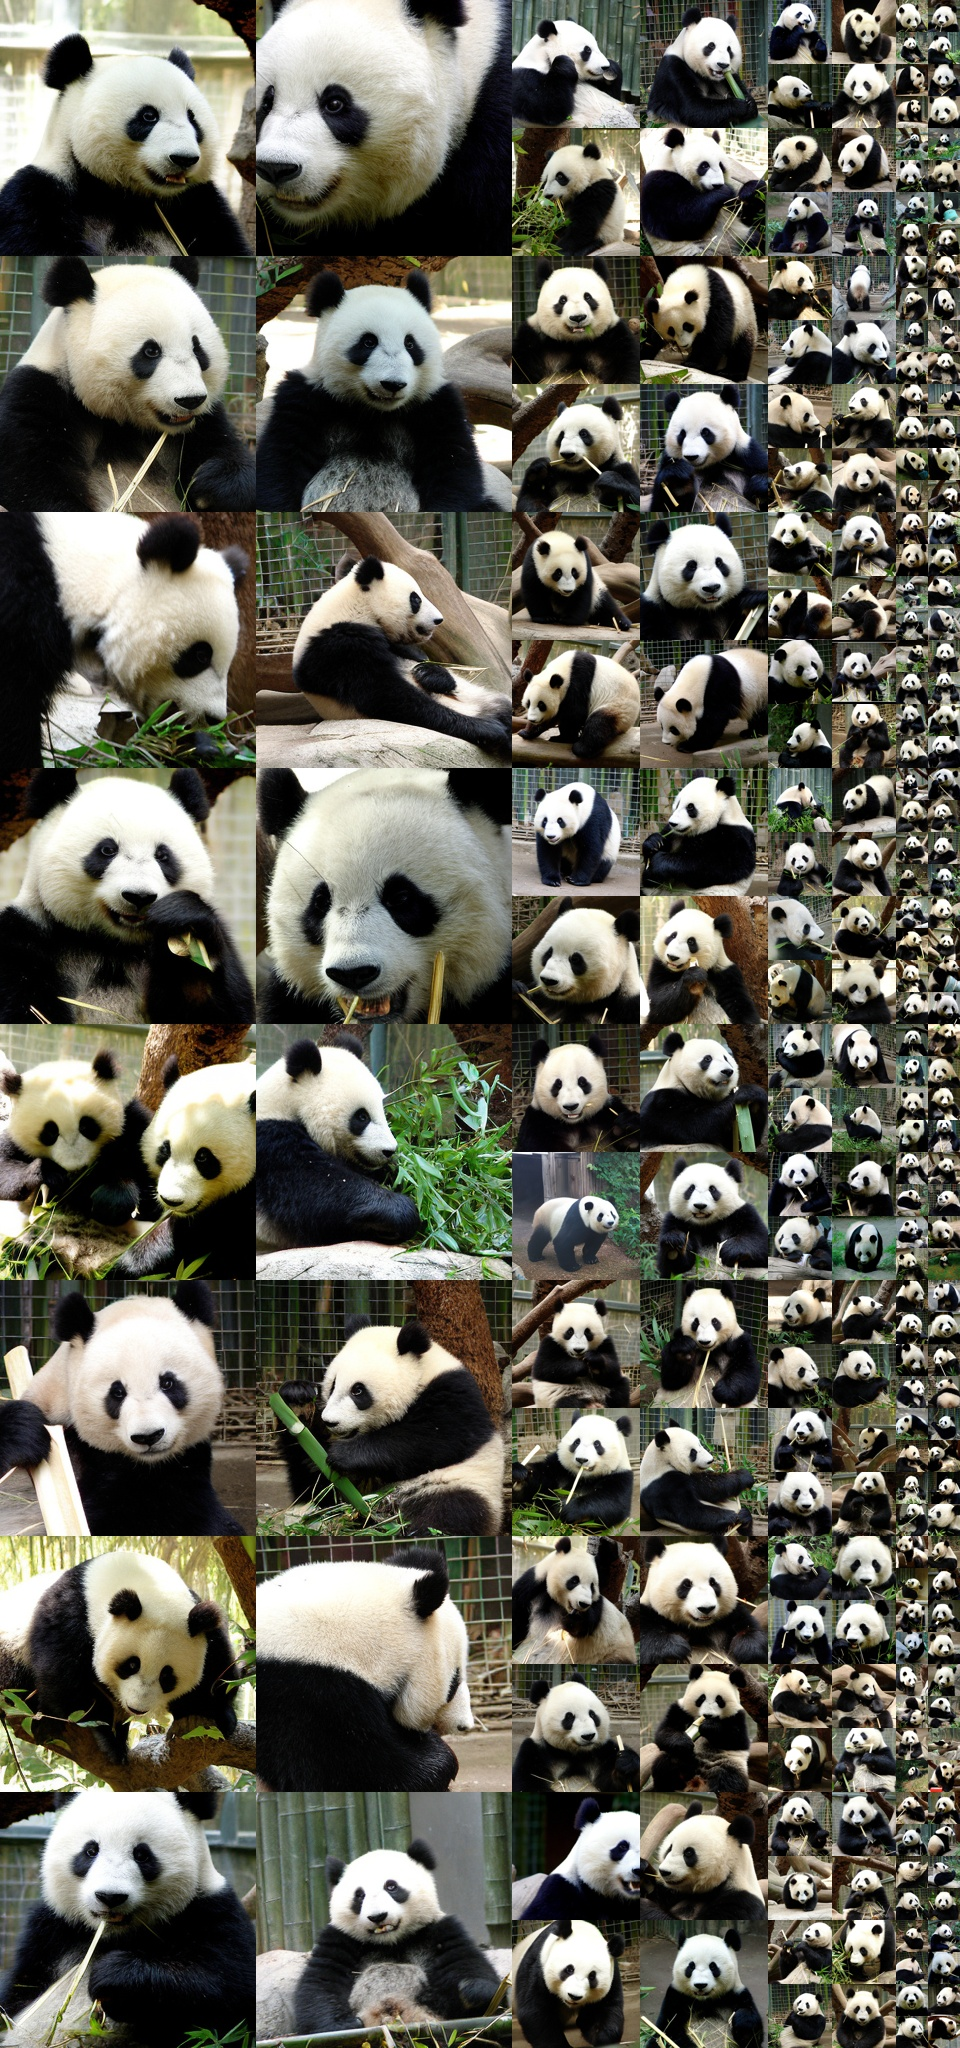
\includegraphics[width=\linewidth]{figs/xl256_388_cfg2.0.jpg}
\caption{\textbf{Uncurated $256\times256$ CausalFusion-XL samples.} \\Classifier-free guidance scale = 2.0\\Class label = ``giant panda" (388)}\vspace{-2mm}
\label{fig:samples256_3}
\end{figure}

\begin{figure}\centering
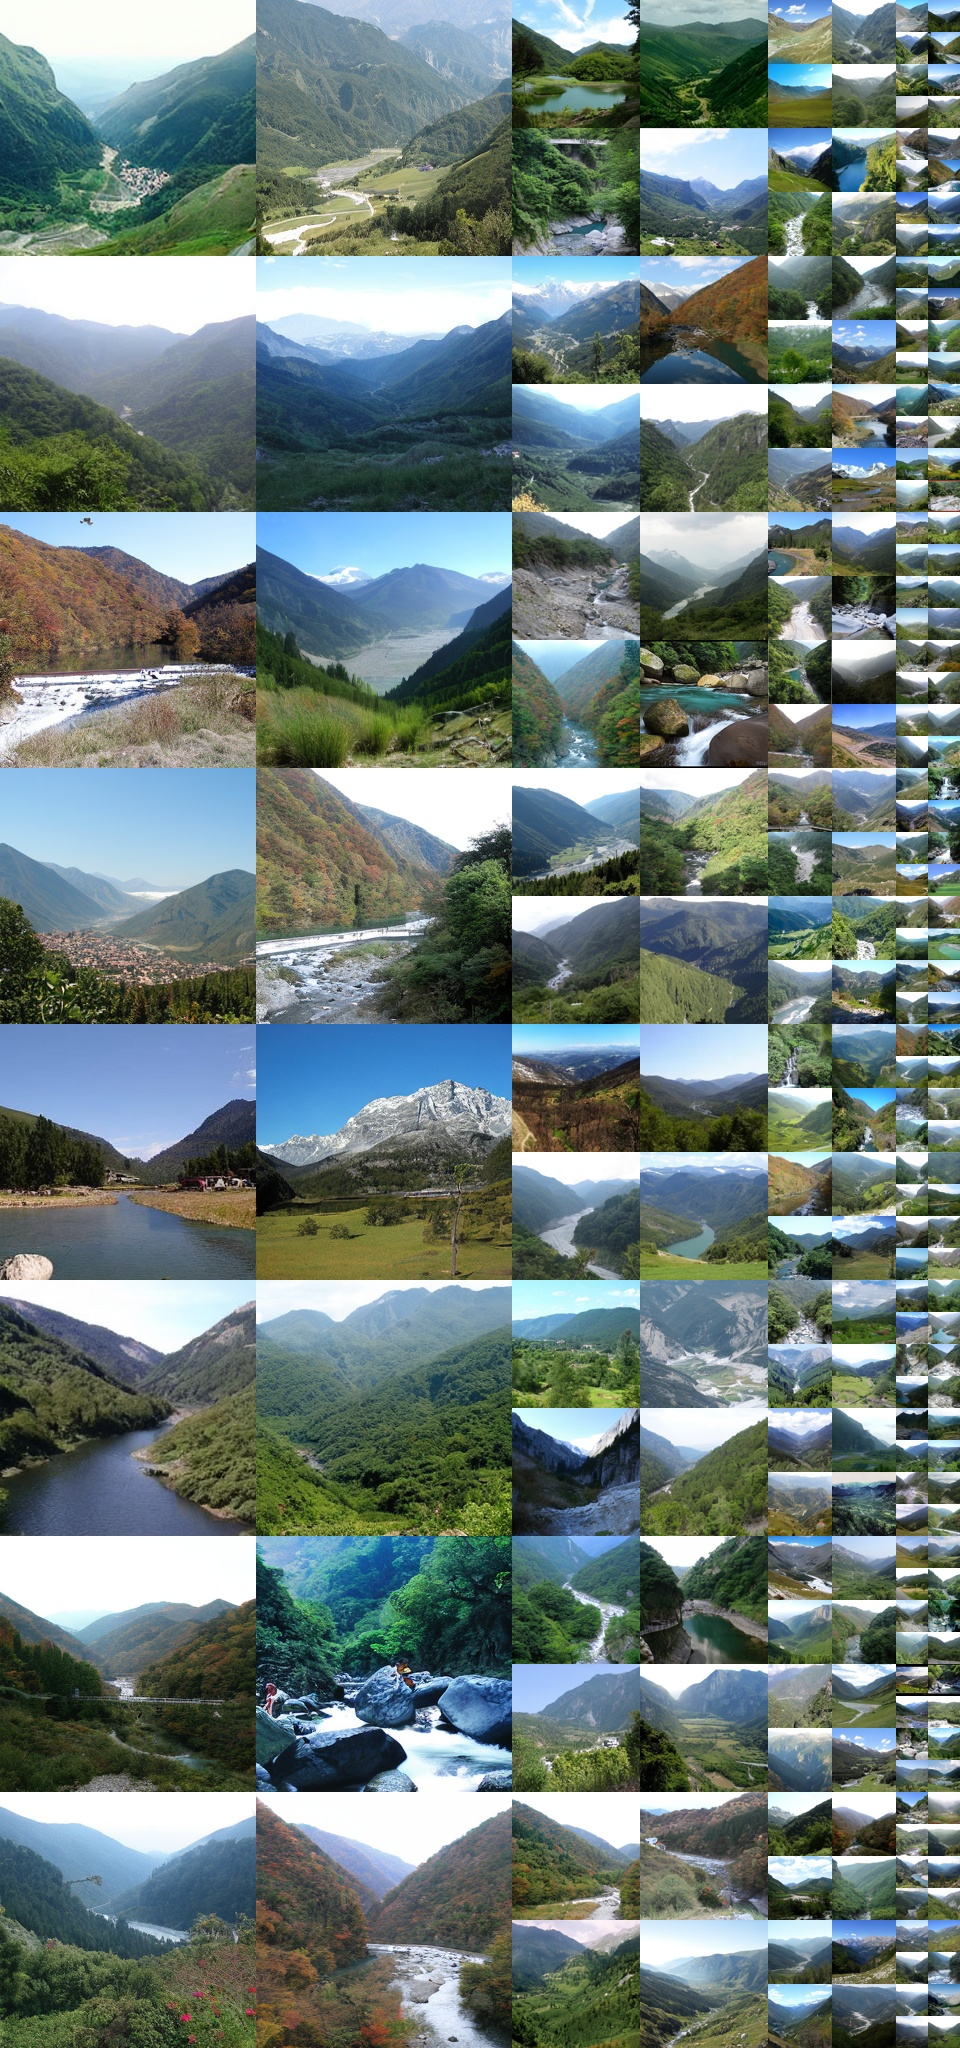
\includegraphics[width=\linewidth]{figs/xl256_979_cfg2.0.jpg}
\caption{\textbf{Uncurated $256\times256$ CausalFusion-XL samples.} \\Classifier-free guidance scale = 2.0\\Class label = ``valley" (979)}\vspace{-2mm}
\label{fig:samples256_4}
\end{figure}


\begin{figure}\centering
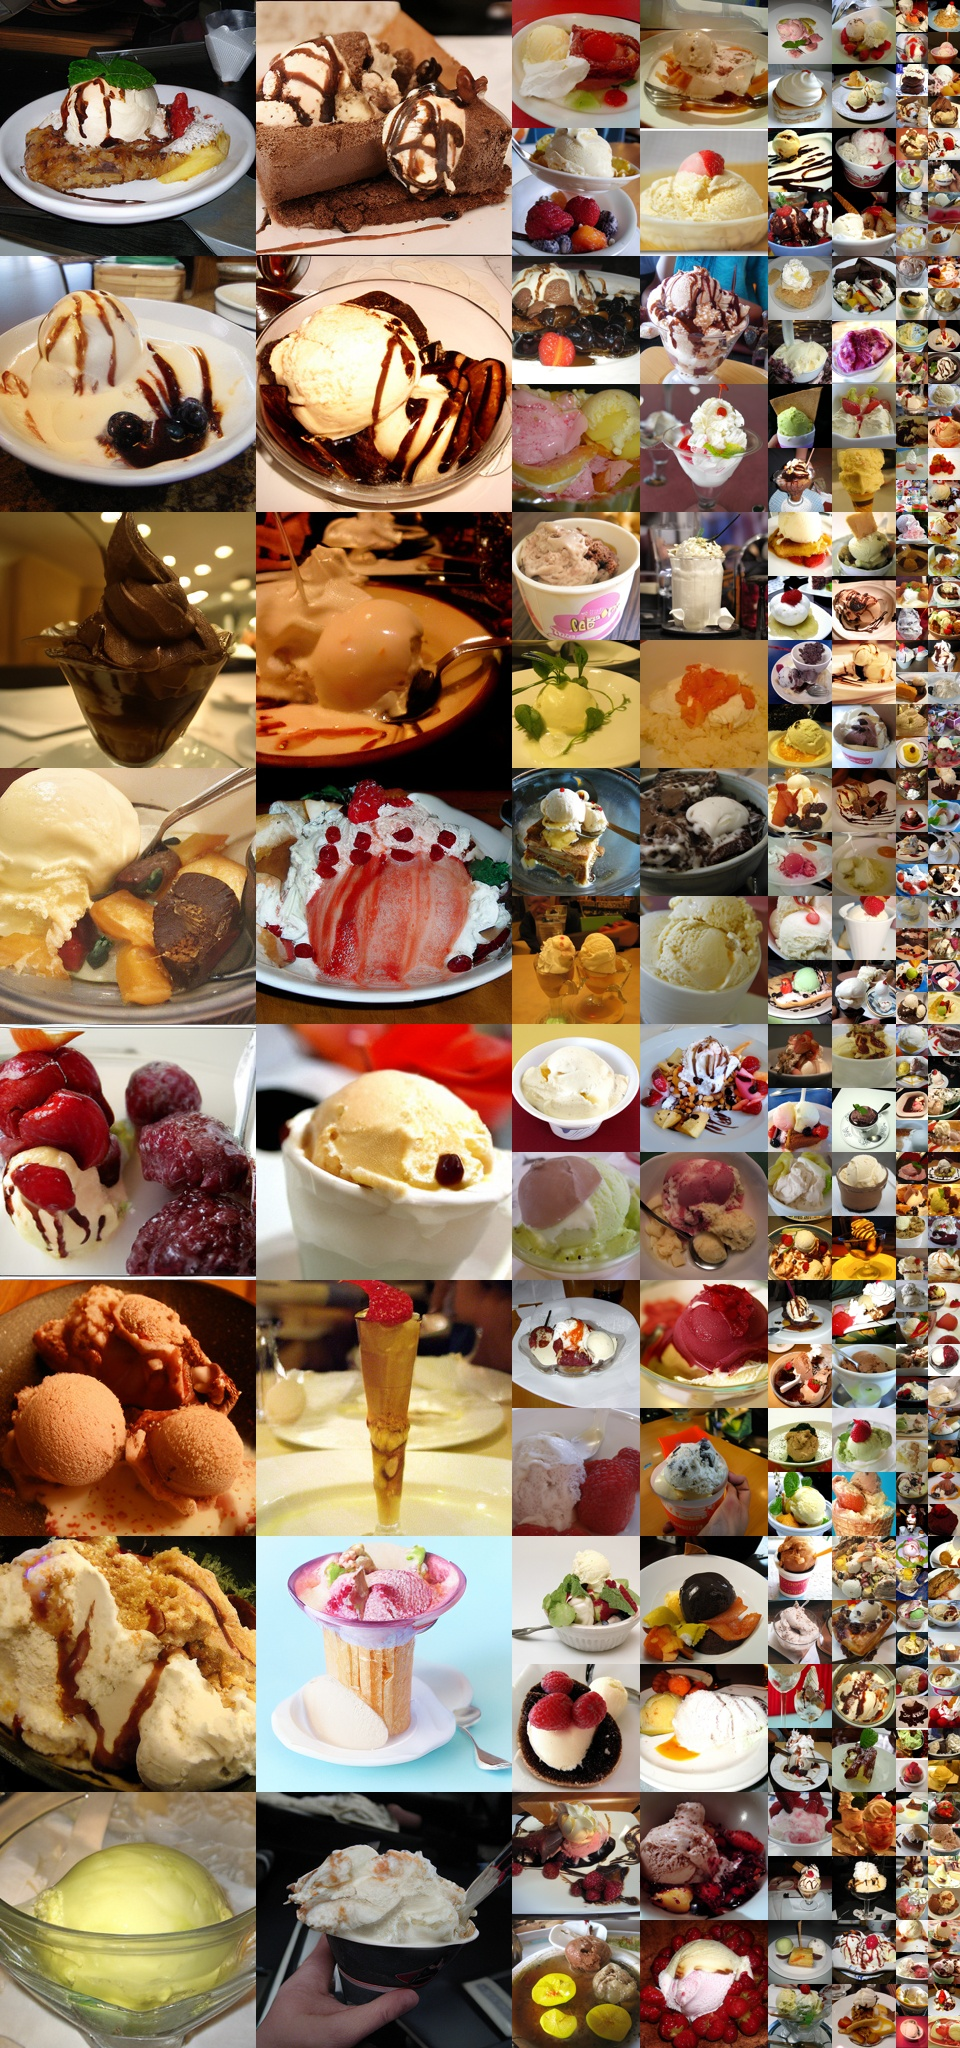
\includegraphics[width=\linewidth]{figs/xl256_928_cfg1.5.jpg}
\caption{\textbf{Uncurated $256\times256$ CausalFusion-XL samples.} \\Classifier-free guidance scale = 1.5\\Class label = ``ice cream" (928)}\vspace{-2mm}
\label{fig:samples256_5}
\end{figure}


\begin{figure}\centering
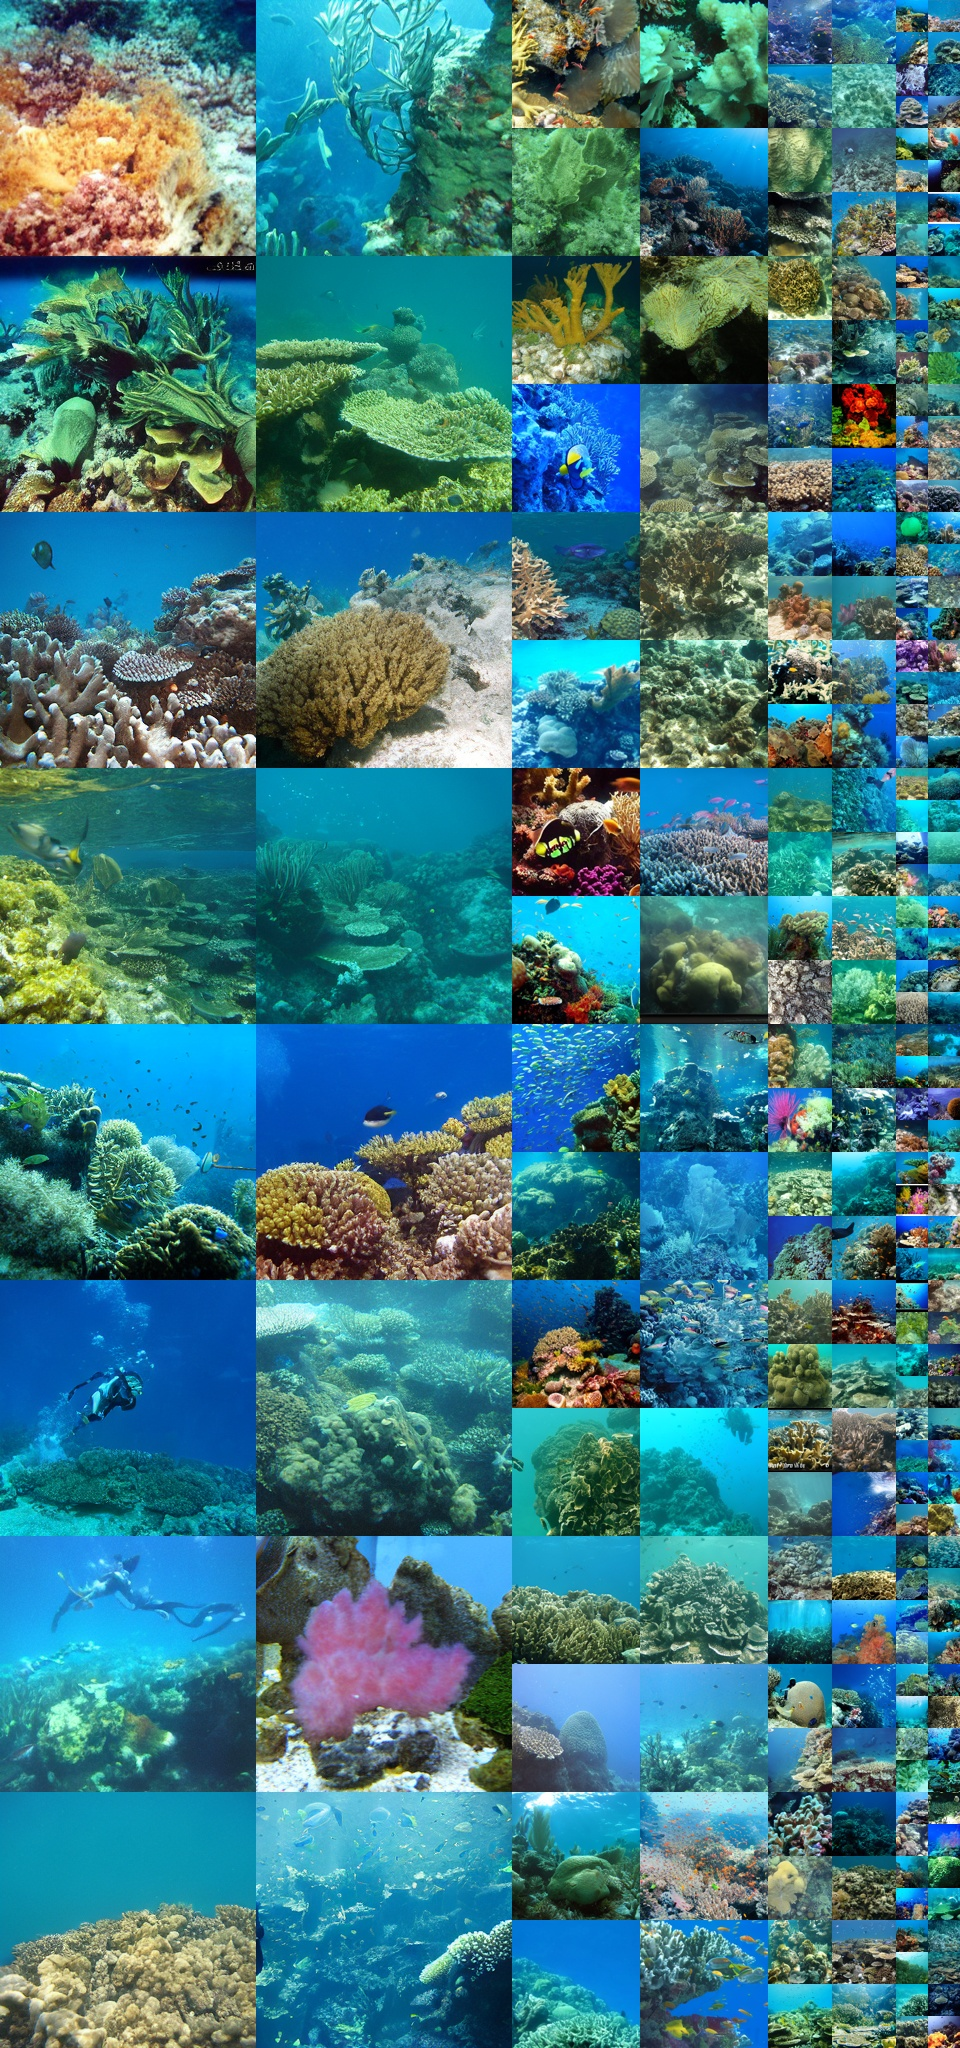
\includegraphics[width=\linewidth]{figs/xl256_973_cfg1.5.jpg}
\caption{\textbf{Uncurated $256\times256$ CausalFusion-XL samples.} \\Classifier-free guidance scale = 1.5\\Class label = ``coral reef" (973)}\vspace{-2mm}
\label{fig:samples256_6}
\end{figure}
